% Options for packages loaded elsewhere
\PassOptionsToPackage{unicode}{hyperref}
\PassOptionsToPackage{hyphens}{url}
\PassOptionsToPackage{dvipsnames,svgnames,x11names}{xcolor}
\documentclass[
  italian,
  10pt,
]{book}
\usepackage{xcolor}
\usepackage[papersize={6in,9in},inner=0.75in,outer=0.5in,top=0.7in,bottom=0.7in]{geometry}
\usepackage{amsmath,amssymb}
\setcounter{secnumdepth}{-\maxdimen} % remove section numbering
\usepackage{iftex}
\ifPDFTeX
  \usepackage[T1]{fontenc}
  \usepackage[utf8]{inputenc}
  \usepackage{textcomp} % provide euro and other symbols
\else % if luatex or xetex
  \usepackage{unicode-math} % this also loads fontspec
  \defaultfontfeatures{Scale=MatchLowercase}
  \defaultfontfeatures[\rmfamily]{Ligatures=TeX,Scale=1}
\fi
\usepackage{lmodern}
\ifPDFTeX\else
  % xetex/luatex font selection
\fi
% Use upquote if available, for straight quotes in verbatim environments
\IfFileExists{upquote.sty}{\usepackage{upquote}}{}
\IfFileExists{microtype.sty}{% use microtype if available
  \usepackage[]{microtype}
  \UseMicrotypeSet[protrusion]{basicmath} % disable protrusion for tt fonts
}{}
\makeatletter
\@ifundefined{KOMAClassName}{% if non-KOMA class
  \IfFileExists{parskip.sty}{%
    \usepackage{parskip}
  }{% else
    \setlength{\parindent}{0pt}
    \setlength{\parskip}{6pt plus 2pt minus 1pt}}
}{% if KOMA class
  \KOMAoptions{parskip=half}}
\makeatother
\usepackage{color}
\usepackage{fancyvrb}
\newcommand{\VerbBar}{|}
\newcommand{\VERB}{\Verb[commandchars=\\\{\}]}
\DefineVerbatimEnvironment{Highlighting}{Verbatim}{commandchars=\\\{\}}
% Add ',fontsize=\small' for more characters per line
\usepackage{framed}
\definecolor{shadecolor}{RGB}{248,248,248}
\newenvironment{Shaded}{\begin{snugshade}}{\end{snugshade}}
\newcommand{\AlertTok}[1]{\textcolor[rgb]{0.94,0.16,0.16}{#1}}
\newcommand{\AnnotationTok}[1]{\textcolor[rgb]{0.56,0.35,0.01}{\textbf{\textit{#1}}}}
\newcommand{\AttributeTok}[1]{\textcolor[rgb]{0.13,0.29,0.53}{#1}}
\newcommand{\BaseNTok}[1]{\textcolor[rgb]{0.00,0.00,0.81}{#1}}
\newcommand{\BuiltInTok}[1]{#1}
\newcommand{\CharTok}[1]{\textcolor[rgb]{0.31,0.60,0.02}{#1}}
\newcommand{\CommentTok}[1]{\textcolor[rgb]{0.56,0.35,0.01}{\textit{#1}}}
\newcommand{\CommentVarTok}[1]{\textcolor[rgb]{0.56,0.35,0.01}{\textbf{\textit{#1}}}}
\newcommand{\ConstantTok}[1]{\textcolor[rgb]{0.56,0.35,0.01}{#1}}
\newcommand{\ControlFlowTok}[1]{\textcolor[rgb]{0.13,0.29,0.53}{\textbf{#1}}}
\newcommand{\DataTypeTok}[1]{\textcolor[rgb]{0.13,0.29,0.53}{#1}}
\newcommand{\DecValTok}[1]{\textcolor[rgb]{0.00,0.00,0.81}{#1}}
\newcommand{\DocumentationTok}[1]{\textcolor[rgb]{0.56,0.35,0.01}{\textbf{\textit{#1}}}}
\newcommand{\ErrorTok}[1]{\textcolor[rgb]{0.64,0.00,0.00}{\textbf{#1}}}
\newcommand{\ExtensionTok}[1]{#1}
\newcommand{\FloatTok}[1]{\textcolor[rgb]{0.00,0.00,0.81}{#1}}
\newcommand{\FunctionTok}[1]{\textcolor[rgb]{0.13,0.29,0.53}{\textbf{#1}}}
\newcommand{\ImportTok}[1]{#1}
\newcommand{\InformationTok}[1]{\textcolor[rgb]{0.56,0.35,0.01}{\textbf{\textit{#1}}}}
\newcommand{\KeywordTok}[1]{\textcolor[rgb]{0.13,0.29,0.53}{\textbf{#1}}}
\newcommand{\NormalTok}[1]{#1}
\newcommand{\OperatorTok}[1]{\textcolor[rgb]{0.81,0.36,0.00}{\textbf{#1}}}
\newcommand{\OtherTok}[1]{\textcolor[rgb]{0.56,0.35,0.01}{#1}}
\newcommand{\PreprocessorTok}[1]{\textcolor[rgb]{0.56,0.35,0.01}{\textit{#1}}}
\newcommand{\RegionMarkerTok}[1]{#1}
\newcommand{\SpecialCharTok}[1]{\textcolor[rgb]{0.81,0.36,0.00}{\textbf{#1}}}
\newcommand{\SpecialStringTok}[1]{\textcolor[rgb]{0.31,0.60,0.02}{#1}}
\newcommand{\StringTok}[1]{\textcolor[rgb]{0.31,0.60,0.02}{#1}}
\newcommand{\VariableTok}[1]{\textcolor[rgb]{0.00,0.00,0.00}{#1}}
\newcommand{\VerbatimStringTok}[1]{\textcolor[rgb]{0.31,0.60,0.02}{#1}}
\newcommand{\WarningTok}[1]{\textcolor[rgb]{0.56,0.35,0.01}{\textbf{\textit{#1}}}}
\usepackage{longtable,booktabs,array}
\usepackage{caption}
\captionsetup[table]{skip=6pt}
\newcounter{none} % for unnumbered tables
\usepackage{calc} % for calculating minipage widths
% Correct order of tables after \paragraph or \subparagraph
\usepackage{etoolbox}
\makeatletter
\patchcmd\longtable{\par}{\if@noskipsec\mbox{}\fi\par}{}{}
\makeatother
\usepackage{graphicx}
\makeatletter
\newsavebox\pandoc@box
\newcommand*\pandocbounded[1]{% scales image to fit in text height/width
  \sbox\pandoc@box{#1}%
  \Gscale@div\@tempa{\textheight}{\dimexpr\ht\pandoc@box+\dp\pandoc@box\relax}%
  \Gscale@div\@tempb{\linewidth}{\wd\pandoc@box}%
  \ifdim\@tempb\p@<\@tempa\p@\let\@tempa\@tempb\fi% select the smaller of both
  \ifdim\@tempa\p@<\p@\scalebox{\@tempa}{\usebox\pandoc@box}%
  \else\usebox{\pandoc@box}%
  \fi%
}
% Set default figure placement to htbp
\def\fps@figure{htbp}
\makeatother
\ifLuaTeX
\usepackage[bidi=basic,shorthands=off]{babel}
\else
\usepackage[bidi=default,shorthands=off]{babel}
\fi
\ifLuaTeX
  \usepackage{selnolig} % disable illegal ligatures
\fi
\setlength{\emergencystretch}{3em} % prevent overfull lines
\providecommand{\tightlist}{%
  \setlength{\itemsep}{0pt}\setlength{\parskip}{0pt}}
\usepackage{fvextra}
\usepackage{float}
\usepackage{xurl}
\usepackage[htt]{hyphenat}
\DefineVerbatimEnvironment{Highlighting}{Verbatim}{breaklines,breakanywhere,fontsize=\small,commandchars=\\\{\}}
\floatplacement{figure}{H}
\setlength{\emergencystretch}{8em}
\sloppy
\usepackage{fancyhdr}
\pagestyle{fancy}
\fancyhf{}
\fancyfoot[C]{\thepage}
\renewcommand{\headrulewidth}{0pt}
\renewcommand{\footrulewidth}{0pt}
\fancypagestyle{plain}{%
  \fancyhf{}
  \fancyfoot[C]{\thepage}
  \renewcommand{\headrulewidth}{0pt}
  \renewcommand{\footrulewidth}{0pt}
}
\usepackage{bookmark}
\IfFileExists{xurl.sty}{\usepackage{xurl}}{} % add URL line breaks if available
\urlstyle{same}
% fallback for those not using the hyperref driver hyperxmp:
\makeatletter
\@ifundefined{xmpquote}{\newcommand{\xmpquote}[1]{#1}}{}
\makeatother
\hypersetup{
  pdftitle={Quaderno AI},
  pdfauthor={Andrea Merlin},
  pdflang={it},
  colorlinks=true,
  linkcolor={blue},
  filecolor={Maroon},
  citecolor={Blue},
  urlcolor={blue},
  pdfcreator={LaTeX via pandoc}}

\title{Quaderno AI}
\usepackage{etoolbox}
\makeatletter
\providecommand{\subtitle}[1]{% add subtitle to \maketitle
  \apptocmd{\@title}{\par {\large #1 \par}}{}{}
}
\makeatother
\subtitle{Concetti, strumenti e percorsi pratici per lo sviluppo
software con AI}
\author{Andrea Merlin}
\date{Numero 1 - Novembre 2026}

\begin{document}
\frontmatter
\maketitle

{
\setcounter{tocdepth}{1}
\tableofcontents
}
\mainmatter
\chapter{Capitolo 3}\label{capitolo-3}

\section{GitHub Spec Kit: sviluppo guidato dalle specifiche con esempi
in
C\#}\label{github-spec-kit-sviluppo-guidato-dalle-specifiche-con-esempi-in-c}

\textbf{Abstract.} Nei primi due capitoli abbiamo costruito software ``a
mano'': scrivevamo il codice e, al massimo, lo descrivevamo mentre lo
producevamo. Esiste però un approccio diverso e sempre più diffuso:
\textbf{capovolgere la piramide} e partire dalla \emph{specifica} --- il
\emph{cosa} e il \emph{perché} --- per poi derivare piano, task e codice
in modo strutturato. \textbf{GitHub Spec Kit} è il toolkit open source
che rende questo approccio concreto per gli agenti di codifica AI. In
questo capitolo capiremo come funziona, ne esploreremo comandi, template
e meccanismi, e lo applicheremo per intero a una feature reale in
\textbf{C\# e .NET 10}.

\subsection{Cosa imparerai in questo
capitolo}\label{cosa-imparerai-in-questo-capitolo}

Al termine della lettura e della pratica saprai:

\begin{itemize}
\tightlist
\item
  spiegare cos'è lo \textbf{spec-driven development} e perché inverte il
  rapporto tradizionale tra specifica e codice;
\item
  installare Spec Kit (CLI \texttt{specify} + integrazione con GitHub
  Copilot o altri agenti);
\item
  orientarti nella struttura di un progetto Spec Kit
  (\texttt{.specify/}, \texttt{specs/}, template, file di stato);
\item
  usare il \textbf{workflow completo}: constitution, specify, clarify,
  plan, checklist, tasks, analyze, implement, polish e converge;
\item
  leggere e compilare i \textbf{template ufficiali} (spec, plan, tasks,
  checklist, constitution);
\item
  applicare l'intero flusso a una feature \textbf{C\#} (una Minimal API
  ASP.NET Core con EF Core), dalla specifica al codice funzionante;
\item
  integrare Spec Kit con \textbf{VS Code e Copilot} e automatizzare i
  controlli in \textbf{CI/CD};
\item
  riconoscere le \textbf{best practice} e gli errori comuni.
\end{itemize}

\subsection{Prerequisiti}\label{prerequisiti}

\begin{itemize}
\tightlist
\item
  .NET SDK 10 e un editor (VS Code con GitHub Copilot, oppure un altro
  agente supportato);
\item
  Python 3.11+ e \texttt{uv} per installare il CLI (vedremo come);
\item
  familiarità con C\# e ASP.NET Core (per l'esempio pratico);
\item
  nessuna conoscenza pregressa di Spec Kit: è l'oggetto di questo
  capitolo.
\end{itemize}

\subsection{Una nota sulla versione}\label{una-nota-sulla-versione}

Spec Kit è in rapida evoluzione: i nomi dei comandi, i percorsi e i
template cambiano tra una versione e l'altra. Questo capitolo usa gli
esempi di comando con trattino (\texttt{/speckit-specify},
\texttt{/speckit-plan}) e descrive la directory \texttt{specs/} per le
feature e lo stato in \texttt{.specify/feature.json}. La sintassi
effettivamente invocabile dipende dall'agente e dalle skill generate
dall'integrazione: fai riferimento ai comandi presenti nel progetto,
senza dedurre dalla punteggiatura che una forma sia necessariamente
obsoleta.

\section{3.1 Lo spec-driven development: invertire la
piramide}\label{lo-spec-driven-development-invertire-la-piramide}

Prima di parlare dello strumento, capiamo la \textbf{filosofia} che lo
anima. GitHub Spec Kit è l'implementazione pratica dello
\emph{Specification-Driven Development} (SDD), un approccio che cambia
il ruolo della specifica nel ciclo di vita del software.

\subsection{3.1.1 Il potere invertito}\label{il-potere-invertito}

Per decenni il codice è stato il re. Le specifiche servivano il codice:
si scrivevano documenti di requisiti per guidare lo sviluppo, e li si
\textbf{scartava} appena cominciava il ``vero lavoro''. Il PRD (Product
Requirements Document) diventava rapidamente obsoleto, il design doc
finiva in un cassetto, e la fonte di verità rimaneva, di fatto, solo il
codice.

Lo spec-driven development inverte questa gerarchia: \textbf{la
specifica è la fonte di verità}, e il codice è una sua
\textbf{derivazione}. La specifica non è un artefatto usa-e-getta, ma un
documento vivo che viene portato avanti attraverso la pianificazione,
l'implementazione e la convergenza finale.

\subsection{3.1.2 Perché proprio adesso}\label{perchuxe9-proprio-adesso}

Tre fattori rendono questo approccio possibile (e conveniente) oggi,
quando in passato era impraticabile:

\begin{enumerate}
\def\labelenumi{\arabic{enumi}.}
\tightlist
\item
  \textbf{Gli agenti AI possono scrivere molto codice in fretta.} Il
  collo di bottiglia non è più digitare il codice, ma decidere
  \emph{cosa} deve fare. Investire tempo nella specifica diventa
  l'investimento a più alto rendimento.
\item
  \textbf{Gli LLM lavorano bene con strutture.} Un template ben
  progettato ``guida'' il modello verso output di qualità costante,
  riducendo divagazioni e dettagli prematuri.
\item
  \textbf{I team sono distribuiti e asincroni.} Una specifica
  versionata, rivista e approvata diventa il contratto condiviso tra chi
  definisce e chi implementa --- umano o agente che sia.
\end{enumerate}

\subsection{3.1.3 L'idea in una frase}\label{lidea-in-una-frase}

\begin{quote}
Definisci \textbf{cosa} costruire e \textbf{perché}, poi trasforma la
specifica in un piano, in task e in codice funzionante.
\end{quote}

Tutto il resto --- comandi, template, checklist --- è al servizio di
questa frase.

\subsection{3.1.4 Il flusso SDD in
pratica}\label{il-flusso-sdd-in-pratica}

Il flusso parte da un'idea, spesso vaga e incompleta:

\begin{enumerate}
\def\labelenumi{\arabic{enumi}.}
\tightlist
\item
  \textbf{Specifica.} Attraverso un dialogo con l'agente, l'idea diventa
  una specifica strutturata: user story prioritarie, criteri di
  accettazione, requisiti funzionali, entità, criteri di successo
  misurabili.
\item
  \textbf{Chiarimento.} Le ambiguità vengono esplicitate e risolte (o
  marcate come \texttt{{[}NEEDS\ CLARIFICATION{]}}).
\item
  \textbf{Piano.} La specifica diventa un piano tecnico: stack,
  architettura, modello dati, contratti.
\item
  \textbf{Task.} Il piano viene scomposto in task ordinati per
  dipendenza, raggruppati per user story.
\item
  \textbf{Implementazione.} I task vengono eseguiti nell'ordine giusto.
\item
  \textbf{Convergenza.} Il codice viene confrontato con la specifica: se
  manca qualcosa, si aggiungono task e si itera finché non c'è
  convergenza.
\end{enumerate}

Ciò che richiedeva giorni di riunioni e documentazione si comprime in
ore di lavoro focalizzato. E, a differenza del passato, gli artefatti
non vengono scartati: restano, versionati, come documentazione viva del
sistema.

\subsection{3.1.5 Il ruolo dei template}\label{il-ruolo-dei-template}

La qualità dell'output dipende in modo cruciale dai \textbf{template}.
Un buon template è, di fatto, un \emph{prompt strutturato} che vincola
il modello in modi produttivi:

\begin{itemize}
\tightlist
\item
  \textbf{impedisce i dettagli implementativi prematuri} (la specifica
  non deve dire ``usa React'', deve dire ``l'utente deve vedere
  aggiornamenti in tempo reale'');
\item
  \textbf{forza i marcatori di incertezza}
  (\texttt{{[}NEEDS\ CLARIFICATION{]}}) invece di lasciare che il
  modello inventi;
\item
  \textbf{include checklist} che funzionano come ``unit test'' per la
  specifica;
\item
  \textbf{impone gate di conformità} ai principi del progetto (la
  \emph{constitution}).
\end{itemize}

Vedremo ciascuno di questi meccanismi in dettaglio nelle prossime
sezioni, perché sono il cuore di Spec Kit.

\subsection{3.1.6 Cosa NON è lo SDD}\label{cosa-non-uxe8-lo-sdd}

Per evitare fraintendimenti:

\begin{itemize}
\tightlist
\item
  non è ``scrivere documenti invece di codice'': è scrivere
  \textbf{prima} i documenti giusti, per scrivere \textbf{meglio} il
  codice dopo;
\item
  non elimina la revisione umana: la sposta, anzi, più a monte, dove
  costa meno;
\item
  non è un processo a cascata rigido: le fasi sono iterative (si può
  tornare indietro e rivedere la specifica);
\item
  non è legato a un linguaggio: funziona con C\#, Python, TypeScript,
  qualunque stack.
\end{itemize}

\section{3.2 Cos'è GitHub Spec Kit}\label{cosuxe8-github-spec-kit}

GitHub Spec Kit è un \textbf{toolkit open source} (repository
\texttt{github/spec-kit}, licenza MIT) che fornisce agli agenti di
codifica AI \emph{processi strutturati}, \emph{template riutilizzabili}
e \emph{risultati documentati}. Non è un framework applicativo né un
linguaggio: è un \textbf{livello di metodo} che si appoggia ai coding
agent esistenti (GitHub Copilot, Claude Code, Cursor e altri).

\subsection{3.2.1 I tre processi pronti
all'uso}\label{i-tre-processi-pronti-alluso}

Spec Kit offre tre punti di ingresso indipendenti --- non fasi
obbligatorie di un unico processo:

{\def\LTcaptype{none} % do not increment counter
\begin{longtable}[]{@{}
  >{\raggedright\arraybackslash}p{(\linewidth - 4\tabcolsep) * \real{0.4167}}
  >{\raggedright\arraybackslash}p{(\linewidth - 4\tabcolsep) * \real{0.2778}}
  >{\raggedright\arraybackslash}p{(\linewidth - 4\tabcolsep) * \real{0.3056}}@{}}
\toprule\noalign{}
\begin{minipage}[b]{\linewidth}\raggedright
Cosa ti serve
\end{minipage} & \begin{minipage}[b]{\linewidth}\raggedright
Processo
\end{minipage} & \begin{minipage}[b]{\linewidth}\raggedright
Risultato
\end{minipage} \\
\midrule\noalign{}
\endhead
\bottomrule\noalign{}
\endlastfoot
Costruire una feature o un'app & \textbf{Spec-Driven Development}
(incluso nel core) & Una specifica portata attraverso piano,
implementazione e convergenza \\
Diagnosticare e riparare un comportamento rotto & \textbf{Bug fixing}
(estensione) & Una causa valutata, una correzione mirata e una verifica
registrata \\
Decidere se un'idea merita investimento & \textbf{Idea assessment}
(estensione) & Una decisione motivata: \texttt{go},
\texttt{needs-clarification} o \texttt{kill} \\
\end{longtable}
}

In questo capitolo ci concentriamo sul processo principale, lo
\textbf{SDD}; nelle sezioni finali accenniamo agli altri due, che
seguono la stessa filosofia.

\subsection{3.2.2 Le capabilities: un toolkit
componibile}\label{le-capabilities-un-toolkit-componibile}

Oltre ai processi, Spec Kit espone un insieme di meccanismi componibili:

\begin{itemize}
\tightlist
\item
  \textbf{Integration} --- collegamento ai diversi coding agent
  (Copilot, Claude Code, Cursor, ecc.);
\item
  \textbf{Extension} --- aggiunta di comandi, gate di qualità o processi
  interi;
\item
  \textbf{Preset} --- adattamento di template, comandi e terminologia
  agli standard del team;
\item
  \textbf{Workflow} --- automazione di prompt, comandi, gate e task di
  shell;
\item
  \textbf{Bundle} --- pacchetti riutilizzabili di estensioni, preset e
  workflow (per ruoli o team);
\item
  \textbf{Catalog} --- catalogo di componenti della comunità, con la
  possibilità di ospitarne di privati;
\item
  \textbf{Project-local override} --- sostituzione di un singolo
  template in un progetto.
\end{itemize}

Questa componibilità è ciò che distingue Spec Kit da una semplice
raccolta di prompt: puoi partire con il processo pronto, adattarlo al
tuo team e persino costruirne uno tuo.

\subsection{3.2.3 Come si usa, in estrema
sintesi}\label{come-si-usa-in-estrema-sintesi}

\begin{enumerate}
\def\labelenumi{\arabic{enumi}.}
\tightlist
\item
  Si installa il \textbf{CLI} (\texttt{specify}) con
  \texttt{uv\ tool\ install\ specify-cli}.
\item
  Si inizializza un progetto con
  \texttt{specify\ init\ \textless{}nome\textgreater{}\ -\/-integration\ copilot}.
\item
  Si apre il progetto nell'agente e si invocano i \textbf{comandi}
  (\texttt{/speckit-specify}, \texttt{/speckit-plan}, \ldots)
  \textbf{nella chat dell'agente}, uno alla volta, rivedendo ogni
  risultato prima di proseguire.
\end{enumerate}

Il CLI fa il lavoro ``di terra'' (scaffolding, controlli dei
prerequisiti, gestione di estensioni e cataloghi); i comandi esposti
dall'integrazione fanno il lavoro ``di testa'', guidando l'agente nella
produzione degli artefatti.

\subsection{3.2.4 Una breve storia}\label{una-breve-storia}

Spec Kit nasce dall'esperienza di \textbf{GitHub Next} e dal progetto
precedente noto come \emph{Specify}, poi evoluto e donato come progetto
open source dell'organizzazione \texttt{github}. I comandi disponibili e
la loro sintassi dipendono dall'integrazione e dalle skill che questa
genera per l'agente: nelle sezioni seguenti usiamo la forma con trattino
mostrata dall'integrazione dell'esempio. Se un progetto espone una forma
diversa, va seguita quella effettivamente generata; la punteggiatura da
sola non indica che si tratti di una generazione precedente.

\subsection{3.2.5 Perché dovrebbe
interessarti}\label{perchuxe9-dovrebbe-interessarti}

Se sviluppi con un coding agent, Spec Kit risponde a tre domande
ricorrenti:

\begin{itemize}
\tightlist
\item
  ``Come faccio a far produrre all'agente \textbf{esattamente ciò che
  voglio}, e non qualcosa di plausibile ma sbagliato?'' --- con una
  specifica strutturata e rivista;
\item
  ``Come \textbf{traccio} il lavoro e lo rendo revisionabile da un
  team?'' --- con artefatti versionati in \texttt{specs/};
\item
  ``Come impongo gli \textbf{standard} del mio team all'agente?'' ---
  con la constitution, i preset e le checklist.
\end{itemize}

È, in sintesi, il modo per passare da ``chiedo una cosa alla volta
all'agente'' a ``dirigo un processo di sviluppo documentato e
ripetibile''.

\section{3.3 Installazione e
inizializzazione}\label{installazione-e-inizializzazione}

Spec Kit ha due componenti da installare: il \textbf{CLI} (uno strumento
da terminale) e l'\textbf{integrazione} con il tuo coding agent (i
comandi \texttt{/speckit-*}).

\subsection{3.3.1 I prerequisiti}\label{i-prerequisiti}

Ti servono:

\begin{itemize}
\tightlist
\item
  \textbf{Python 3.11 o superiore};
\item
  \textbf{\texttt{uv}}, il gestore di pacchetti Python veloce (il CLI
  \texttt{specify} è distribuito come pacchetto Python);
\item
  un coding agent supportato: GitHub Copilot, Claude Code, Cursor,
  Windsurf, Qoder, Amazon Q, Antigravity, Crush, Gemini CLI, Kilo Code,
  OpenCode, Roo Code e altri;
\item
  sistema operativo Linux, macOS o Windows.
\end{itemize}

\subsection{3.3.2 Installare il CLI}\label{installare-il-cli}

\begin{Shaded}
\begin{Highlighting}[]
\ExtensionTok{uv}\NormalTok{ tool install specify{-}cli}
\end{Highlighting}
\end{Shaded}

Il comando installa l'eseguibile \texttt{specify} nel tuo ambiente.
Verifica l'installazione:

\begin{Shaded}
\begin{Highlighting}[]
\ExtensionTok{specify} \AttributeTok{{-}{-}version}
\end{Highlighting}
\end{Shaded}

\begin{quote}
\textbf{Nota.} \texttt{uv} è il metodo di installazione raccomandato
nella documentazione ufficiale. Esistono anche altri installer (release
pinnate, pacchetti per CI); per questo capitolo usiamo \texttt{uv}, che
è il percorso più semplice.
\end{quote}

\subsection{3.3.3 Inizializzare un
progetto}\label{inizializzare-un-progetto}

\begin{Shaded}
\begin{Highlighting}[]
\ExtensionTok{specify}\NormalTok{ init taskify }\AttributeTok{{-}{-}integration}\NormalTok{ copilot}
\BuiltInTok{cd}\NormalTok{ taskify}
\end{Highlighting}
\end{Shaded}

Il comando:

\begin{enumerate}
\def\labelenumi{\arabic{enumi}.}
\tightlist
\item
  crea la cartella del progetto;
\item
  genera la struttura di base di Spec Kit (\texttt{.specify/} con
  template, constitution e configurazione);
\item
  configura l'\textbf{integrazione} scelta
  (\texttt{-\/-integration\ copilot}): per Copilot, crea le skill
  \texttt{/speckit-*} nella cartella \texttt{.github/} (o equivalente),
  pronte per essere invocate nella chat dell'agente;
\item
  se interattivo, ti chiede alcune preferenze (per esempio la variante
  degli script di automazione: Bash, PowerShell o Python).
\end{enumerate}

Dopo \texttt{init}, apri la cartella nel tuo agente (per esempio
\texttt{code\ taskify} in VS Code) e sei pronto a lavorare.

\subsection{3.3.4 Inizializzare in un progetto
esistente}\label{inizializzare-in-un-progetto-esistente}

Spec Kit può essere adottato anche in un repository già esistente: la
procedura è la stessa, eseguita dentro la cartella del progetto:

\begin{Shaded}
\begin{Highlighting}[]
\BuiltInTok{cd}\NormalTok{ mio{-}progetto{-}esistente}
\ExtensionTok{specify}\NormalTok{ init . }\AttributeTok{{-}{-}integration}\NormalTok{ copilot}
\end{Highlighting}
\end{Shaded}

In questo caso Spec Kit aggiunge la sua struttura senza toccare il
codice esistente, e puoi iniziare a usare il flusso SDD per le
\textbf{nuove} feature (e, con le guide appropriate, per far evolvere le
specifiche esistenti).

\subsection{\texorpdfstring{3.3.5 Le opzioni di
\texttt{init}}{3.3.5 Le opzioni di init}}\label{le-opzioni-di-init}

\texttt{specify\ init} accetta opzioni utili:

{\def\LTcaptype{none} % do not increment counter
\begin{longtable}[]{@{}
  >{\raggedright\arraybackslash}p{(\linewidth - 2\tabcolsep) * \real{0.5625}}
  >{\raggedright\arraybackslash}p{(\linewidth - 2\tabcolsep) * \real{0.4375}}@{}}
\toprule\noalign{}
\begin{minipage}[b]{\linewidth}\raggedright
Opzione
\end{minipage} & \begin{minipage}[b]{\linewidth}\raggedright
Scopo
\end{minipage} \\
\midrule\noalign{}
\endhead
\bottomrule\noalign{}
\endlastfoot
\texttt{-\/-integration\ \textless{}agente\textgreater{}} & Configura
l'agente (copilot, claude, cursor, \ldots) \\
\texttt{-\/-script\ sh\textbackslash{}\textbar{}ps\textbackslash{}\textbar{}py}
& Sceglie la variante degli script di automazione \\
\texttt{-\/-non-interactive} & Esecuzione senza prompt (per CI) \\
\end{longtable}
}

In modalità non interattiva (nessun terminale, o
\texttt{-\/-non-interactive}), Spec Kit sceglie automaticamente una
variante di script adatta al sistema operativo.

\subsection{3.3.6 Aggiornare}\label{aggiornare}

Per aggiornare un'installazione esistente:

\begin{Shaded}
\begin{Highlighting}[]
\ExtensionTok{uv}\NormalTok{ tool upgrade specify{-}cli}
\end{Highlighting}
\end{Shaded}

L'upgrade del CLI non sovrascrive i tuoi template e le tue specifiche:
aggiorna il tool, lasciando intatti gli artefatti del progetto (che
restano versionati in Git).

\subsection{3.3.7 Cosa succede alla prima
esecuzione}\label{cosa-succede-alla-prima-esecuzione}

Alla prima invocazione di un comando \texttt{/speckit-*}, l'agente legge
la configurazione del progetto (\texttt{.specify/}) e i template, e
produce il primo artefatto (per esempio
\texttt{specs/\textless{}numero\textgreater{}-\textless{}slug\textgreater{}/spec.md}).
Non c'è un ``server'' da avviare: tutto avviene tramite file Markdown
versionati e il dialogo con l'agente. Questa semplicità --- nessun
servizio, nessun database --- è parte del fascino dello strumento.

\section{3.4 La struttura di un progetto Spec
Kit}\label{la-struttura-di-un-progetto-spec-kit}

Capire la struttura delle cartelle è essenziale per orientarsi e per
personalizzare il toolkit. Ecco l'anatomia di un progetto inizializzato.

\subsection{3.4.1 La struttura d'insieme}\label{la-struttura-dinsieme}

\begin{figure}
\centering
\pandocbounded{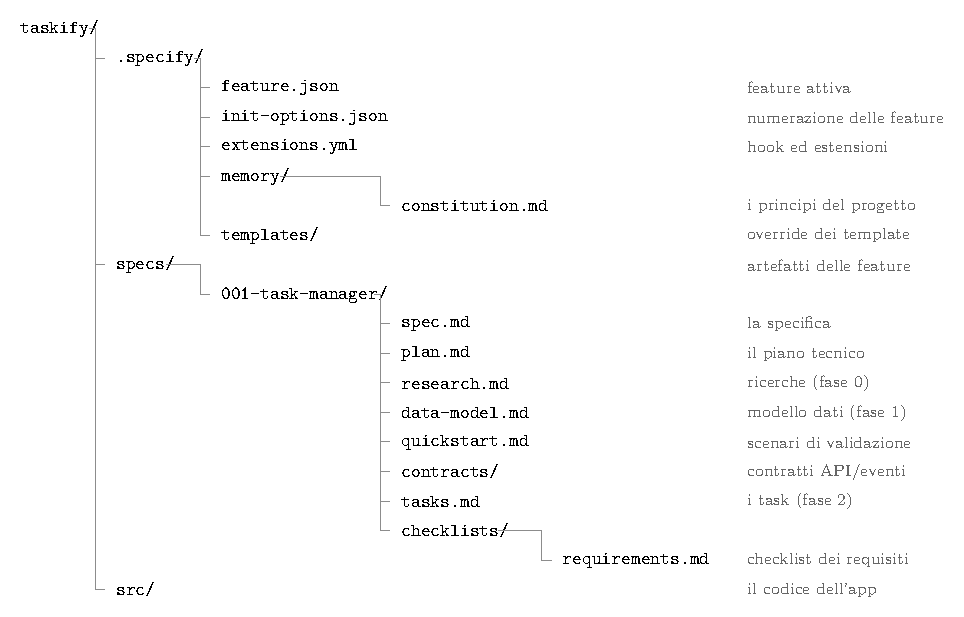
\includegraphics[keepaspectratio,alt={Anatomia di un
progetto Spec Kit dopo specify init}]{figure/struttura-spec-kit.pdf}}
\caption{Anatomia di un progetto Spec Kit dopo
\protect\texttt{specify\ init}}
\end{figure}

\subsection{\texorpdfstring{3.4.2 La cartella
\texttt{.specify/}}{3.4.2 La cartella .specify/}}\label{la-cartella-.specify}

È il ``cervello'' della configurazione. Contiene:

\begin{itemize}
\tightlist
\item
  \textbf{\texttt{feature.json}} --- registra quale feature è
  \textbf{attiva} in questo momento. I comandi \texttt{/speckit-*}
  risolvono la feature da questo stato, \textbf{non} dal branch Git
  corrente. È ciò che permette di lavorare su una feature senza fare
  \texttt{git\ checkout}, e di cambiarla aggiornando il file (o la
  variabile d'ambiente \texttt{SPECIFY\_FEATURE\_DIRECTORY}).
\item
  \textbf{\texttt{init-options.json}} --- conserva le scelte fatte in
  fase di \texttt{init}, in particolare la \textbf{numerazione} delle
  feature (\texttt{feature\_numbering}): da qui deriva il nome della
  cartella, per esempio \texttt{003-user-auth}.
\item
  \textbf{\texttt{memory/constitution.md}} --- i principi stabili del
  progetto, modificabili solo attraverso le regole di governance. È la
  ``legge'' che i comandi di piano e implementazione devono rispettare.
\item
  \textbf{\texttt{templates/}} --- se presenti, i template in questa
  cartella \textbf{sostituiscono} quelli di default per il singolo
  progetto (project-local override).
\item
  \textbf{\texttt{extensions.yml}} --- (facoltativo) registra estensioni
  e \textbf{hook}, cioè azioni da eseguire prima o dopo i comandi (per
  esempio creare il branch Git all'avvio di una feature).
\end{itemize}

\subsection{\texorpdfstring{3.4.3 La cartella
\texttt{specs/}}{3.4.3 La cartella specs/}}\label{la-cartella-specs}

È dove vivono gli \textbf{artefatti di ogni feature}. Ogni feature ha
una cartella con un nome del tipo
\texttt{\textless{}prefisso\textgreater{}-\textless{}slug\textgreater{}}
(per esempio \texttt{001-task-manager}), che contiene i file prodotti
dai comandi:

{\def\LTcaptype{none} % do not increment counter
\begin{longtable}[]{@{}
  >{\raggedright\arraybackslash}p{(\linewidth - 2\tabcolsep) * \real{0.4615}}
  >{\raggedright\arraybackslash}p{(\linewidth - 2\tabcolsep) * \real{0.5385}}@{}}
\toprule\noalign{}
\begin{minipage}[b]{\linewidth}\raggedright
Artefatto
\end{minipage} & \begin{minipage}[b]{\linewidth}\raggedright
Comando e scopo
\end{minipage} \\
\midrule\noalign{}
\endhead
\bottomrule\noalign{}
\endlastfoot
\texttt{spec.md} & \texttt{/speckit-specify}: specifica (cosa e
perché) \\
\texttt{plan.md} & \texttt{/speckit-plan}: piano tecnico (come) \\
\texttt{research.md} & \texttt{/speckit-plan}: ricerche tecniche (fase
0) \\
\texttt{data-model.md} & \texttt{/speckit-plan}: modello dati (fase
1) \\
\texttt{quickstart.md} & \texttt{/speckit-plan}: scenari chiave di
validazione \\
\texttt{contracts/} & \texttt{/speckit-plan}: contratti di endpoint ed
eventi \\
\texttt{tasks.md} & \texttt{/speckit-tasks}: task eseguibili \\
\texttt{checklists/requirements.md} & \texttt{/speckit-specify} e
\texttt{/speckit-clarify}: checklist di qualità dei requisiti \\
\end{longtable}
}

\subsection{3.4.4 Lo stato della feature
attiva}\label{lo-stato-della-feature-attiva}

Il file \texttt{.specify/feature.json} ha una forma simile a:

\begin{Shaded}
\begin{Highlighting}[]
\FunctionTok{\{}
  \DataTypeTok{"feature\_directory"}\FunctionTok{:} \StringTok{"specs/001{-}task{-}manager"}
\FunctionTok{\}}
\end{Highlighting}
\end{Shaded}

Quando invochi \texttt{/speckit-plan} o \texttt{/speckit-tasks}, il
comando legge questo file e sa \textbf{dove} andare a lavorare. È un
dettaglio piccolo ma potente: svincola il flusso dal branch Git e lo
rende deterministico (e più facile da automatizzare in CI).

\subsection{3.4.5 Il codice sorgente}\label{il-codice-sorgente}

Spec Kit non impone una struttura al codice: la struttura del codice
viene decisa \textbf{nel piano} (il file \texttt{plan.md} contiene una
sezione ``Project Structure'' con l'albero delle cartelle scelto). Per
un'applicazione web, per esempio, il piano potrà proporre \texttt{src/}
e \texttt{tests/}, o \texttt{backend/} e \texttt{frontend/}. I task
faranno riferimento a quei percorsi.

\subsection{3.4.6 Dove vengono creati i file: un
riepilogo}\label{dove-vengono-creati-i-file-un-riepilogo}

\begin{itemize}
\tightlist
\item
  \textbf{\texttt{specify\ init}} crea \texttt{.specify/}, i template di
  default e la constitution;
\item
  \textbf{\texttt{/speckit-constitution}} aggiorna
  \texttt{.specify/memory/constitution.md};
\item
  \textbf{\texttt{/speckit-specify}} crea
  \texttt{specs/\textless{}slug\textgreater{}/spec.md} e
  \texttt{checklists/requirements.md};
\item
  \textbf{\texttt{/speckit-plan}} crea \texttt{plan.md},
  \texttt{research.md}, \texttt{data-model.md}, \texttt{quickstart.md} e
  \texttt{contracts/};
\item
  \textbf{\texttt{/speckit-tasks}} crea \texttt{tasks.md};
\item
  \textbf{\texttt{/speckit-implement}} crea il codice sorgente vero e
  proprio.
\end{itemize}

Con questa mappa in testa, il resto del capitolo scorrerà molto più
facilmente.

\section{3.5 Il workflow a colpo
d'occhio}\label{il-workflow-a-colpo-docchio}

Spec Kit definisce due percorsi per lo SDD: uno \textbf{breve} (per
feature piccole) e uno \textbf{completo} (per feature di produzione). In
entrambi i casi, i comandi si invocano \textbf{nella chat dell'agente},
uno alla volta, rivedendo ogni risultato prima di procedere.

\subsection{3.5.1 Il percorso breve}\label{il-percorso-breve}

Per feature piccole o prototipi:

\begin{enumerate}
\def\labelenumi{\arabic{enumi}.}
\tightlist
\item
  \texttt{/speckit-specify} → la specifica (\texttt{spec.md})
\item
  \texttt{/speckit-plan} → il piano tecnico (\texttt{plan.md}, \ldots)
\item
  \texttt{/speckit-tasks} → i task (\texttt{tasks.md})
\item
  \texttt{/speckit-implement} → il codice
\item
  \texttt{/speckit-converge} → verifica della completezza
\end{enumerate}

\subsection{3.5.2 Il percorso completo}\label{il-percorso-completo}

Per feature di produzione, con i gate di qualità:

\begin{enumerate}
\def\labelenumi{\arabic{enumi}.}
\tightlist
\item
  \texttt{/speckit-constitution} (una volta per progetto)
\item
  \texttt{/speckit-specify}
\item
  \texttt{/speckit-clarify} → risolve le ambiguità
\item
  \texttt{/speckit-plan}
\item
  \texttt{/speckit-checklist} → checklist di qualità della specifica
\item
  \texttt{/speckit-tasks}
\item
  \texttt{/speckit-analyze} → verifica di coerenza tra gli artefatti
\item
  \texttt{/speckit-implement}
\item
  \textbf{Polish} → revisione mirata, rifinitura e test del risultato,
  senza ampliare la specifica
\item
  \texttt{/speckit-converge} → verifica della completezza
\end{enumerate}

\textbf{Polish} è un'attività di revisione, non un comando standard di
Spec Kit: si esegue dopo l'implementazione e si ripetono i test prima
della convergenza. Il diagramma mostra i comandi del flusso e perciò non
rappresenta questa attività trasversale. Se l'integrazione offre una
skill dedicata, usane la sintassi generata.

Le fasi aggiuntive (\texttt{clarify}, \texttt{checklist},
\texttt{analyze}) sono \textbf{gate di qualità}: costano poco, si
eseguono in chat e intercettano i problemi prima che diventino codice
sbagliato.

\subsection{3.5.3 Il diagramma del
flusso}\label{il-diagramma-del-flusso}

\begin{figure}
\centering
\pandocbounded{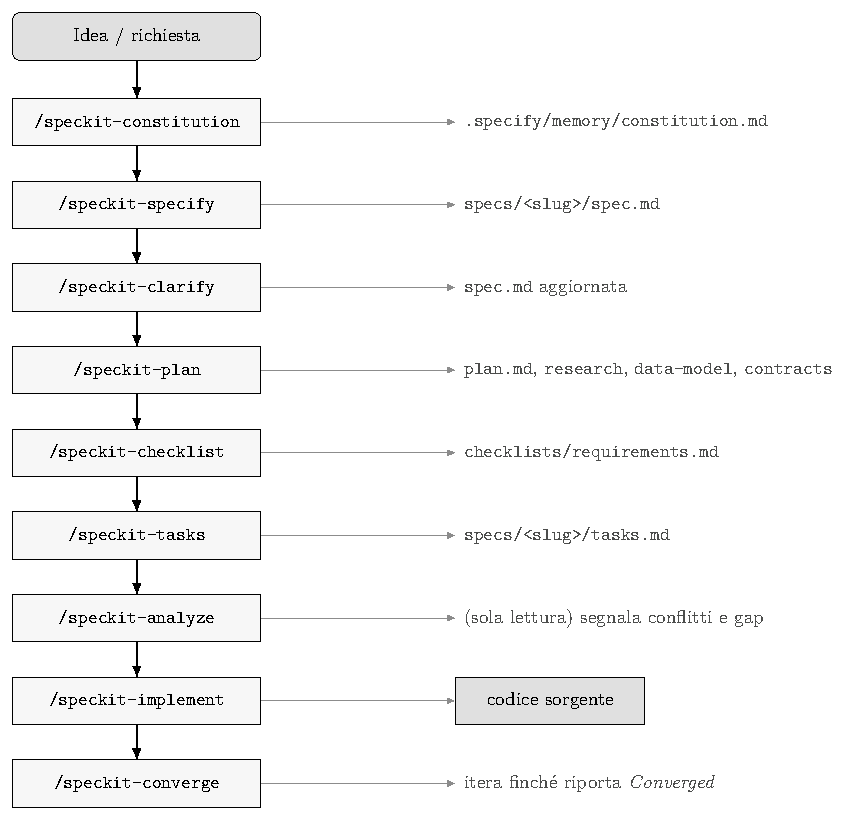
\includegraphics[keepaspectratio,alt={Il flusso completo
di Spec Kit: comandi a sinistra, artefatti prodotti a
destra}]{figure/workflow-flusso.pdf}}
\caption{Il flusso completo di Spec Kit: comandi a sinistra, artefatti
prodotti a destra}
\end{figure}

\subsection{3.5.4 Le regole d'uso}\label{le-regole-duso}

Tre regole fondamentali, ripetute nella documentazione ufficiale:

\begin{enumerate}
\def\labelenumi{\arabic{enumi}.}
\tightlist
\item
  \textbf{Un comando alla volta.} Non incatenare i comandi: esegui
  \texttt{/speckit-specify}, rivedi il risultato, poi passa al
  successivo. Ogni comando dipende dall'output del precedente.
\item
  \textbf{Rivedi prima di proseguire.} Gli artefatti sono tuoi: se la
  specifica non riflette ciò che volevi, correggila (a mano o chiedendo
  all'agente) prima di pianificare.
\item
  \textbf{I comandi si eseguono nella chat, non nel terminale.} Il CLI
  \texttt{specify} serve per \texttt{init}, estensioni e controlli dei
  prerequisiti; i comandi \texttt{/speckit-*} sono skill dell'agente.
\end{enumerate}

\subsection{3.5.5 Cosa produce la
convergenza}\label{cosa-produce-la-convergenza}

L'ultimo comando, \texttt{/speckit-converge}, confronta il
\textbf{codice} con \textbf{spec, plan e task}. Se trova gap
(funzionalità richieste ma non implementate), \textbf{aggiunge nuovi
task} a \texttt{tasks.md}; poi riesegui \texttt{/speckit-implement} e di
nuovo \texttt{/speckit-converge}, finché non riporta \textbf{Converged}.
È il meccanismo che chiude il cerchio e garantisce che il codice
corrisponda alla specifica --- non ``più o meno'', ma in modo
verificabile.

\section{3.6 La Constitution: i principi del
progetto}\label{la-constitution-i-principi-del-progetto}

La \textbf{constitution} è la base di tutto: un insieme di principi che
governano il modo in cui le specifiche diventano codice. Vive in
\texttt{.specify/memory/constitution.md} e viene letta dai comandi di
piano e implementazione, che devono \textbf{conformarsi} ad essa.

\subsection{3.6.1 Cosa contiene}\label{cosa-contiene}

Il template della constitution definisce una struttura chiara:

\begin{Shaded}
\begin{Highlighting}[]
\FunctionTok{\# [Nome progetto] Constitution}

\FunctionTok{\#\# Core Principles}
\FunctionTok{\#\#\# I. [Nome principio]}
\CommentTok{[}\OtherTok{Descrizione}\CommentTok{]}

\FunctionTok{\#\#\# II. [Nome principio]}
\CommentTok{[}\OtherTok{Descrizione}\CommentTok{]}
\NormalTok{...}

\FunctionTok{\#\# [Sezione aggiuntiva, es. Security Requirements]}
\CommentTok{[}\OtherTok{Contenuto}\CommentTok{]}

\FunctionTok{\#\# [Sezione aggiuntiva, es. Development Workflow]}
\CommentTok{[}\OtherTok{Contenuto}\CommentTok{]}

\FunctionTok{\#\# Governance}
\CommentTok{[}\OtherTok{Regole di governo: la constitution prevale sulle altre pratiche, ecc.}\CommentTok{]}

\NormalTok{**Version**: ... | **Ratified**: ... | **Last Amended**: ...}
\end{Highlighting}
\end{Shaded}

I \textbf{Core Principles} sono articoli numerati; le sezioni aggiuntive
coprono vincoli specifici (sicurezza, performance, workflow); la sezione
\textbf{Governance} stabilisce come si modifica la constitution e che
essa prevale sulle altre pratiche.

\subsection{3.6.2 Un esempio per un progetto
.NET}\label{un-esempio-per-un-progetto-.net}

Ecco una constitution realistica per il nostro progetto di esempio (la
vedremo applicata nel resto del capitolo):

\begin{Shaded}
\begin{Highlighting}[]
\FunctionTok{\# Taskify Constitution}

\FunctionTok{\#\# Core Principles}

\FunctionTok{\#\#\# I. Test{-}First (NON NEGOZIABILE)}
\NormalTok{TDD obbligatorio: i test si scrivono prima dell\textquotesingle{}implementazione,}
\NormalTok{devono fallire, e solo dopo si implementa (Red{-}Green{-}Refactor).}

\FunctionTok{\#\#\# II. Semplicità}
\NormalTok{Parti dalla soluzione più semplice. Niente astrazioni speculative:}
\NormalTok{introduci un\textquotesingle{}astrazione solo quando serve davvero (YAGNI).}

\FunctionTok{\#\#\# III. Validazione degli input}
\NormalTok{Ogni input esterno deve essere validato e restituire errori chiari.}
\NormalTok{Nessuna eccezione non gestita verso il chiamante.}

\FunctionTok{\#\#\# IV. API REST coerenti}
\NormalTok{Gli endpoint usano JSON, verbi HTTP corretti e codici di stato}
\NormalTok{semantici. Le risorse sono al plurale (/tasks).}
\NormalTok{Per una transizione di dominio modellata come comando esplicito, è}
\NormalTok{ammesso un endpoint }\InformationTok{\textasciigrave{}POST\textasciigrave{}}\NormalTok{ dedicato (per esempio }\InformationTok{\textasciigrave{}/tasks/\{id\}/complete\textasciigrave{}}\NormalTok{),}
\NormalTok{purché il piano ne motivi la scelta e ne documenti gli effetti.}

\FunctionTok{\#\# Security Requirements}
\SpecialStringTok{{-} }\NormalTok{Nessun segreto nel codice o nei file di configurazione versionati.}
\SpecialStringTok{{-} }\NormalTok{Le operazioni distruttive richiedono conferma esplicita.}

\FunctionTok{\#\# Development Workflow}
\SpecialStringTok{{-} }\NormalTok{Ogni feature passa da specifica, piano e task prima del codice.}
\SpecialStringTok{{-} }\NormalTok{Le modifiche sono riviste tramite pull request.}

\FunctionTok{\#\# Governance}
\NormalTok{La constitution prevale sulle altre pratiche. Può essere emendata, ma le}
\NormalTok{modifiche richiedono documentazione, approvazione e un piano di migrazione;}
\NormalTok{gli emendamenti sono versionati e aggiornano le date indicate in calce.}

\NormalTok{**Version**: 1.0.0 | **Ratified**: 2026{-}01{-}15 | **Last Amended**: 2026{-}01{-}15}
\end{Highlighting}
\end{Shaded}

\subsection{3.6.3 Come viene usata}\label{come-viene-usata}

La constitution non è un documento ornamentale. Durante il piano, il
comando \texttt{/speckit-plan} esegue un \textbf{Constitution Check}:
una lista di gate che il piano deve superare prima di procedere. Per
esempio, con la constitution sopra, il piano dovrà dimostrare:

\begin{itemize}
\tightlist
\item
  che i test sono previsti \textbf{prima} dell'implementazione
  (Test-First);
\item
  che l'architettura scelta è la più \textbf{semplice} (niente
  microservizi se basta una Minimal API);
\item
  che la \textbf{validazione} degli input è prevista;
\item
  che le API seguono le \textbf{convenzioni REST} dichiarate.
\end{itemize}

Se il piano viola un principio (per esempio introduce un'astrazione
ingiustificata), deve \textbf{giustificarlo} esplicitamente nella
sezione ``Complexity Tracking'', oppure semplificare.

\subsection{\texorpdfstring{3.6.4 La creazione con
\texttt{/speckit-constitution}}{3.6.4 La creazione con /speckit-constitution}}\label{la-creazione-con-speckit-constitution}

Il comando si invoca \textbf{una volta per progetto}, con una
descrizione dei principi voluti:

\begin{Shaded}
\begin{Highlighting}[]
\NormalTok{/speckit{-}constitution Taskify è un progetto "security{-}first": tutti gli input}
\NormalTok{vanno validati. Usiamo una Minimal API .NET con SQLite. I test sono obbligatori}
\NormalTok{e vanno scritti prima del codice.}
\end{Highlighting}
\end{Shaded}

L'agente produce (o aggiorna) \texttt{.specify/memory/constitution.md}
traducendo la descrizione in principi strutturati. Puoi poi
\textbf{modificarla a mano}: è un normale file Markdown versionato.

\subsection{3.6.5 Perché è potente}\label{perchuxe9-uxe8-potente}

La constitution è ciò che rende il comportamento dell'agente
\textbf{coerente nel tempo e tra i membri del team}. Senza di essa, ogni
feature potrebbe essere implementata con scelte diverse; con essa, tutte
le feature rispettano gli stessi principi, e le violazioni devono essere
esplicite e motivate. In un'organizzazione, è il modo per codificare gli
standard architetturali e farli rispettare --- non per buona volontà, ma
per \textbf{gate}.

\section{\texorpdfstring{3.7 \texttt{/speckit-specify}: dalla richiesta
alla
specifica}{3.7 /speckit-specify: dalla richiesta alla specifica}}\label{speckit-specify-dalla-richiesta-alla-specifica}

Il primo comando del flusso trasforma una descrizione in linguaggio
naturale in una \textbf{specifica strutturata}. È il momento in cui
l'idea vaga diventa un documento con requisiti, scenari e criteri di
successo.

\subsection{3.7.1 Come si invoca}\label{come-si-invoca}

\begin{Shaded}
\begin{Highlighting}[]
\NormalTok{/speckit{-}specify Crea una Task Manager API dove gli utenti possono creare task,}
\NormalTok{elencarli con un filtro per stato, completarli ed eliminarli.}
\end{Highlighting}
\end{Shaded}

Il comando:

\begin{enumerate}
\def\labelenumi{\arabic{enumi}.}
\tightlist
\item
  determina il nome e il numero della feature (per esempio
  \texttt{001-task-manager});
\item
  crea la cartella \texttt{specs/001-task-manager/};
\item
  copia il \textbf{template di specifica} in \texttt{spec.md} e lo
  compila con i requisiti estratti dalla richiesta;
\item
  genera la \textbf{checklist di qualità} in
  \texttt{checklists/requirements.md}.
\end{enumerate}

\subsection{\texorpdfstring{3.7.2 La struttura di
\texttt{spec.md}}{3.7.2 La struttura di spec.md}}\label{la-struttura-di-spec.md}

Il template di specifica è il cuore del comando. Le sue sezioni
principali:

{\def\LTcaptype{none} % do not increment counter
\begin{longtable}[]{@{}
  >{\raggedright\arraybackslash}p{(\linewidth - 2\tabcolsep) * \real{0.5625}}
  >{\raggedright\arraybackslash}p{(\linewidth - 2\tabcolsep) * \real{0.4375}}@{}}
\toprule\noalign{}
\begin{minipage}[b]{\linewidth}\raggedright
Sezione
\end{minipage} & \begin{minipage}[b]{\linewidth}\raggedright
Scopo
\end{minipage} \\
\midrule\noalign{}
\endhead
\bottomrule\noalign{}
\endlastfoot
\textbf{User Scenarios \& Testing} & User story prioritarie (P1, P2,
\ldots), ciascuna con test indipendente e scenari Given/When/Then \\
\textbf{Edge Cases} & Condizioni limite e scenari d'errore \\
\textbf{Requirements} & Requisiti funzionali \texttt{FR-xxx} + entità
chiave \\
\textbf{Success Criteria} & Criteri di successo misurabili
\texttt{SC-xxx}, indipendenti dalla tecnologia \\
\textbf{Assumptions} & Ipotesi ragionevoli quando la richiesta non
specifica dettagli \\
\end{longtable}
}

\subsection{3.7.3 Le user story prioritarie e
indipendenti}\label{le-user-story-prioritarie-e-indipendenti}

La sezione più importante è quella delle user story. Il template impone
due proprietà fondamentali:

\begin{enumerate}
\def\labelenumi{\arabic{enumi}.}
\tightlist
\item
  \textbf{Priorità} --- ogni story ha una priorità (\texttt{P1},
  \texttt{P2}, \texttt{P3}\ldots), con \texttt{P1} la più critica.
\item
  \textbf{Testabilità indipendente} --- ogni story deve poter essere
  sviluppata, testata e dimostrata \textbf{da sola}: se implementi solo
  la \texttt{P1}, hai comunque un MVP che porta valore.
\end{enumerate}

Per ogni story il template chiede:

\begin{itemize}
\tightlist
\item
  una descrizione in linguaggio semplice;
\item
  il \textbf{motivo della priorità};
\item
  un \textbf{test indipendente} (come verificarla da sola);
\item
  gli \textbf{acceptance scenarios} in formato \textbf{Given/When/Then}.
\end{itemize}

\subsection{3.7.4 L'esempio C\#: la
specifica}\label{lesempio-c-la-specifica}

Applichiamo subito il template alla nostra feature. Ecco come appare
\texttt{specs/001-task-manager/spec.md} compilata (mostriamo le parti
essenziali):

\begin{Shaded}
\begin{Highlighting}[]
\FunctionTok{\# Feature Specification: Task Manager API}

\NormalTok{**Feature Branch**: }\InformationTok{\textasciigrave{}001{-}task{-}manager\textasciigrave{}}
\NormalTok{**Status**: Draft}
\NormalTok{**Input**: User description: "Crea una Task Manager API dove gli utenti}
\NormalTok{possono creare task, elencarli con un filtro per stato, completarli ed}
\NormalTok{eliminarli."}

\FunctionTok{\#\# User Scenarios \& Testing}

\FunctionTok{\#\#\# User Story 1 {-} Creare un task (Priority: P1)}

\NormalTok{Un utente crea un task fornendo un titolo e, facoltativamente, una data di}
\NormalTok{scadenza. Il task viene salvato e restituito con il suo identificativo.}

\NormalTok{**Why this priority**: senza la creazione non esiste alcun dato su cui}
\NormalTok{operare: è il fondamento dell\textquotesingle{}intera feature.}

\NormalTok{**Independent Test**: si può verificare con una singola chiamata}
\NormalTok{POST /tasks e la successiva lettura del task creato.}

\NormalTok{**Acceptance Scenarios**:}
\SpecialStringTok{1. }\NormalTok{**Given** nessun task esistente, **When** l\textquotesingle{}utente invia POST /tasks}
\NormalTok{   con un titolo valido, **Then** il task viene creato e restituito con id.}
\SpecialStringTok{2. }\NormalTok{**Given** una richiesta senza titolo, **When** l\textquotesingle{}utente invia POST /tasks,}
\NormalTok{   **Then** il sistema risponde 400 con un messaggio di validazione.}

\NormalTok{{-}{-}{-}}

\FunctionTok{\#\#\# User Story 2 {-} Elencare e filtrare i task (Priority: P2)}

\NormalTok{L\textquotesingle{}utente elenca i task, con un filtro opzionale per stato (open/completed).}

\NormalTok{**Why this priority**: la creazione è inutile senza la possibilità di}
\NormalTok{consultare i task.}

\NormalTok{**Independent Test**: si verifica con GET /tasks e GET /tasks?status=...}

\NormalTok{**Acceptance Scenarios**:}
\SpecialStringTok{1. }\NormalTok{**Given** task esistenti in stati diversi, **When** l\textquotesingle{}utente richiede}
\NormalTok{   GET /tasks?status=open, **Then** riceve solo i task aperti.}

\NormalTok{{-}{-}{-}}

\FunctionTok{\#\#\# User Story 3 {-} Completare ed eliminare (Priority: P3)}

\NormalTok{L\textquotesingle{}utente marca un task come completato o lo elimina.}

\NormalTok{**Why this priority**: chiude il ciclo di vita, ma il sistema è già utile}
\NormalTok{con le prime due story.}

\NormalTok{**Acceptance Scenarios**:}
\SpecialStringTok{1. }\NormalTok{**Given** un task esistente, **When** l\textquotesingle{}utente invia}
\NormalTok{   POST /tasks/\{id\}/complete, **Then** il task risulta completato.}
\SpecialStringTok{2. }\NormalTok{**Given** un task esistente, **When** l\textquotesingle{}utente invia}
\NormalTok{   DELETE /tasks/\{id\}, **Then** il task viene eliminato.}

\FunctionTok{\#\#\# Edge Cases}

\SpecialStringTok{{-} }\NormalTok{Cosa succede se il titolo è vuoto o supera 200 caratteri?}
\SpecialStringTok{{-} }\NormalTok{Cosa succede se si richiede un task con id inesistente?}
\SpecialStringTok{{-} }\NormalTok{Cosa succede se la data di scadenza è nel passato?}

\FunctionTok{\#\# Requirements}

\FunctionTok{\#\#\# Functional Requirements}

\SpecialStringTok{{-} }\NormalTok{**FR{-}001**: Il sistema DEVE permettere di creare un task con titolo}
\NormalTok{  obbligatorio (max 200 caratteri) e data di scadenza opzionale.}
\SpecialStringTok{{-} }\NormalTok{**FR{-}002**: Il sistema DEVE elencare i task, con filtro opzionale per stato.}
\SpecialStringTok{{-} }\NormalTok{**FR{-}003**: Il sistema DEVE permettere di marcare un task come completato.}
\SpecialStringTok{{-} }\NormalTok{**FR{-}004**: Il sistema DEVE permettere di eliminare un task.}
\SpecialStringTok{{-} }\NormalTok{**FR{-}005**: Il sistema DEVE restituire errori chiari in caso di input}
\NormalTok{  non valido o risorsa inesistente.}

\FunctionTok{\#\#\# Key Entities}

\SpecialStringTok{{-} }\NormalTok{**Task**: un\textquotesingle{}attività con titolo, stato (aperto/completato),}
\NormalTok{  data di scadenza opzionale e data di creazione.}

\FunctionTok{\#\# Success Criteria}

\SpecialStringTok{{-} }\NormalTok{**SC{-}001**: una task può essere creata e letta in meno di 100 ms in locale.}
\SpecialStringTok{{-} }\NormalTok{**SC{-}002**: il 100\% degli scenari di accettazione è coperto da test.}
\SpecialStringTok{{-} }\NormalTok{**SC{-}003**: nessuna richiesta valida produce un errore 500.}

\FunctionTok{\#\# Assumptions}

\SpecialStringTok{{-} }\NormalTok{Il primo rilascio non prevede autenticazione: l\textquotesingle{}API è monoutente.}
\SpecialStringTok{{-} }\NormalTok{La persistenza usa un database locale SQLite.}
\SpecialStringTok{{-} }\NormalTok{La paginazione è fuori scope per la v1.}
\end{Highlighting}
\end{Shaded}

\subsection{3.7.5 I punti chiave del
template}\label{i-punti-chiave-del-template}

Osserva come il template \textbf{vincola} il modello:

\begin{itemize}
\tightlist
\item
  i requisiti sono \texttt{FR-xxx} numerati e verificabili, non prosa
  libera;
\item
  le incertezze sono esplicitate (il template prevede il marcatore
  \texttt{{[}NEEDS\ CLARIFICATION{]}} per i requisiti non specificati:
  lo vedremo con \texttt{/speckit-clarify});
\item
  i criteri di successo sono \textbf{misurabili e indipendenti dalla
  tecnologia} (nessun ``usa .NET'': quello appartiene al piano, non alla
  specifica);
\item
  le entità sono descritte \textbf{senza dettagli implementativi}
  (``titolo, stato, scadenza'', non ``tabella SQL con colonna
  VARCHAR(200)'').
\end{itemize}

Questa separazione tra \emph{cosa} (specifica) e \emph{come} (piano) è
il principio più importante dell'intero metodo.

\section{\texorpdfstring{3.8 \texttt{/speckit-clarify}: risolvere le
ambiguità}{3.8 /speckit-clarify: risolvere le ambiguità}}\label{speckit-clarify-risolvere-le-ambiguituxe0}

Dopo la specifica, quasi sempre restano punti oscuri. Il comando
\texttt{/speckit-clarify} li affronta sistematicamente, prima che
diventino decisioni arbitrarie (o bug) in fase di implementazione.

\subsection{3.8.1 Cosa fa}\label{cosa-fa}

\begin{Shaded}
\begin{Highlighting}[]
\NormalTok{/speckit{-}clarify Concentrati sul comportamento dei task: validazione del titolo,}
\NormalTok{gestione degli id inesistenti e semantica del filtro per stato.}
\end{Highlighting}
\end{Shaded}

Il comando:

\begin{enumerate}
\def\labelenumi{\arabic{enumi}.}
\tightlist
\item
  esamina \texttt{spec.md} alla ricerca di ambiguità e punti deboli;
\item
  \textbf{pone domande} all'utente (una alla volta, con opzioni o
  risposte libere);
\item
  aggiorna \texttt{spec.md} con le risposte;
\item
  aggiorna la checklist dei requisiti in
  \texttt{checklists/requirements.md}.
\end{enumerate}

È un dialogo, non un comando ``one-shot'': l'agente fa domande, tu
rispondi, e la specifica si affina.

\subsection{\texorpdfstring{3.8.2 Il marcatore
\texttt{{[}NEEDS\ CLARIFICATION{]}}}{3.8.2 Il marcatore {[}NEEDS CLARIFICATION{]}}}\label{il-marcatore-needs-clarification}

Il template di specifica prevede di marcare esplicitamente ciò che non è
stato specificato. Per esempio:

\begin{Shaded}
\begin{Highlighting}[]
\SpecialStringTok{{-} }\NormalTok{**FR{-}006**: Il sistema DEVE autenticare gli utenti tramite}
  \CommentTok{[}\OtherTok{NEEDS CLARIFICATION: metodo non specificato — email/password, SSO, OAuth?}\CommentTok{]}
\end{Highlighting}
\end{Shaded}

\texttt{/speckit-clarify} è il momento in cui questi marcatori vengono
\textbf{risolti}: la domanda viene posta, la risposta sostituisce il
marcatore. L'alternativa --- lasciare che l'agente inventi una risposta
plausibile --- è esattamente ciò che il metodo vuole evitare.

\subsection{3.8.3 Esempi di domande per la nostra
feature}\label{esempi-di-domande-per-la-nostra-feature}

Per la Task Manager API, domande tipiche di chiarimento:

\begin{itemize}
\tightlist
\item
  ``Il titolo deve avere un limite di lunghezza? Se sì, quale?''
\item
  ``La data di scadenza può essere nel passato?''
\item
  ``Il filtro per stato accetta solo \texttt{open}/\texttt{completed}, o
  anche valori parziali?''
\item
  ``L'eliminazione deve essere fisica (record rimosso) o logica (soft
  delete)?''
\item
  ``Serve una data di completamento registrata quando un task viene
  completato?''
\end{itemize}

Ogni risposta si traduce in un requisito aggiornato o in una nuova voce
nella sezione Edge Cases/Requirements.

\subsection{3.8.4 Quando usarlo}\label{quando-usarlo}

\begin{itemize}
\tightlist
\item
  \textbf{Sempre} nel percorso completo (per feature di produzione);
\item
  per feature piccole e ben definite si può saltare, come previsto dal
  percorso breve;
\item
  in ogni caso, se la specifica contiene
  \texttt{{[}NEEDS\ CLARIFICATION{]}} irrisolti, è un segnale che serve
  un giro di chiarimento.
\end{itemize}

\subsection{3.8.5 Il valore per il team}\label{il-valore-per-il-team}

\texttt{/speckit-clarify} sposta le decisioni di prodotto \textbf{dove
costano meno}: prima di pianificare e molto prima di scrivere codice.
Una domanda risolta nella specifica vale dieci correzioni in code
review. E poiché le risposte finiscono nel \texttt{spec.md} versionato,
restano documentate per chiunque rilegga la feature in futuro.

\section{\texorpdfstring{3.9 \texttt{/speckit-plan}: il piano
tecnico}{3.9 /speckit-plan: il piano tecnico}}\label{speckit-plan-il-piano-tecnico}

Ora che \emph{cosa} costruire è chiaro, \texttt{/speckit-plan} decide
\emph{come}. È il comando che introduce --- finalmente --- la
tecnologia, nel nostro caso \textbf{C\# e .NET}.

\subsection{3.9.1 Come si invoca}\label{come-si-invoca-1}

\begin{Shaded}
\begin{Highlighting}[]
\NormalTok{/speckit{-}plan Usa .NET 10 con una Minimal API ASP.NET Core. Persistenza con}
\NormalTok{Entity Framework Core su SQLite. Test con xUnit.}
\end{Highlighting}
\end{Shaded}

La richiesta di piano fornisce i \textbf{vincoli tecnici} (stack,
librerie, piattaforma). Se qualcosa non è specificato, il comando lo
chiede o lo marca \texttt{NEEDS\ CLARIFICATION}.

\subsection{3.9.2 Le fasi del piano}\label{le-fasi-del-piano}

Il comando lavora in fasi:

\begin{itemize}
\tightlist
\item
  \textbf{Fase 0 --- Ricerca.} Se serve, esplora le opzioni tecniche
  (librerie, pattern) e produce \texttt{research.md}.
\item
  \textbf{Fase 1 --- Progettazione.} Produce \texttt{data-model.md} (le
  entità), \texttt{contracts/} (gli endpoint e i loro contratti),
  \texttt{quickstart.md} (gli scenari chiave di validazione).
\item
  \textbf{Fase 2 --- Piano.} Produce \texttt{plan.md}, il documento
  principale.
\end{itemize}

In più, \textbf{prima della Fase 0} esegue il \textbf{Constitution
Check}: il piano deve rispettare i principi della constitution, oppure
giustificare le violazioni.

\subsection{\texorpdfstring{3.9.3 La struttura di
\texttt{plan.md}}{3.9.3 La struttura di plan.md}}\label{la-struttura-di-plan.md}

Il template di piano ha queste sezioni:

{\def\LTcaptype{none} % do not increment counter
\begin{longtable}[]{@{}
  >{\raggedright\arraybackslash}p{(\linewidth - 2\tabcolsep) * \real{0.4500}}
  >{\raggedright\arraybackslash}p{(\linewidth - 2\tabcolsep) * \real{0.5500}}@{}}
\toprule\noalign{}
\begin{minipage}[b]{\linewidth}\raggedright
Sezione
\end{minipage} & \begin{minipage}[b]{\linewidth}\raggedright
Contenuto
\end{minipage} \\
\midrule\noalign{}
\endhead
\bottomrule\noalign{}
\endlastfoot
\textbf{Summary} & Requisito primario + approccio tecnico scelto \\
\textbf{Technical Context} & Linguaggio, dipendenze, storage, test,
piattaforma, performance, vincoli, scala \\
\textbf{Constitution Check} & I gate derivati dalla constitution \\
\textbf{Project Structure} & Albero delle cartelle del codice
sorgente \\
\textbf{Complexity Tracking} & (solo se serve) giustificazione delle
violazioni di semplicità \\
\end{longtable}
}

\subsection{3.9.4 L'esempio C\#: il piano}\label{lesempio-c-il-piano}

Ecco \texttt{specs/001-task-manager/plan.md} compilata per la nostra
feature:

\begin{Shaded}
\begin{Highlighting}[]
\FunctionTok{\# Implementation Plan: Task Manager API}

\NormalTok{**Branch**: }\InformationTok{\textasciigrave{}001{-}task{-}manager\textasciigrave{}}\NormalTok{ | **Spec**: specs/001{-}task{-}manager/spec.md}

\FunctionTok{\#\# Summary}

\NormalTok{Una Minimal API ASP.NET Core che espone operazioni CRUD su task}
\NormalTok{(creazione, elenco con filtro, completamento, eliminazione), con}
\NormalTok{persistenza su SQLite tramite Entity Framework Core.}

\FunctionTok{\#\# Technical Context}

\NormalTok{**Language/Version**: C\# 14 / .NET 10}
\NormalTok{**Primary Dependencies**: ASP.NET Core (Minimal API),}
\NormalTok{  Microsoft.EntityFrameworkCore.Sqlite}
\NormalTok{**Storage**: SQLite (file locale)}
\NormalTok{**Testing**: xUnit + WebApplicationFactory}
\NormalTok{**Target Platform**: server Windows/Linux/macOS}
\NormalTok{**Project Type**: web{-}service}
\NormalTok{**Performance Goals**: \textless{}100 ms per operazione su set di 10.000 task}
\NormalTok{**Constraints**: nessun servizio esterno, API REST JSON}
\NormalTok{**Scale/Scope**: monoutente, migliaia di task}

\FunctionTok{\#\# Constitution Check}

\SpecialStringTok{{-} }\VariableTok{[x]}\NormalTok{ Test{-}First: i test di accettazione precedono l\textquotesingle{}implementazione}
\SpecialStringTok{{-} }\VariableTok{[x]}\NormalTok{ Semplicità: una sola Minimal API, nessuna astrazione superflua}
\SpecialStringTok{{-} }\VariableTok{[x]}\NormalTok{ Validazione input: DataAnnotations/minimal validation sugli endpoint}
\SpecialStringTok{{-} }\VariableTok{[x]}\NormalTok{ API REST coerenti: risorse al plurale (/tasks), codici di stato semantici; il completamento usa il comando esplicito }\InformationTok{\textasciigrave{}POST /tasks/\{id\}/complete\textasciigrave{}}\NormalTok{, ammesso dalla constitution}

\FunctionTok{\#\# Project Structure}

\NormalTok{src/}
\PreprocessorTok{|}\NormalTok{{-}{-} Taskify.csproj}
\PreprocessorTok{|}\NormalTok{{-}{-} Program.cs            \# bootstrap + endpoint}
\PreprocessorTok{|}\NormalTok{{-}{-} Models/}
\PreprocessorTok{|}\NormalTok{   \textasciigrave{}{-}{-} TaskItem.cs}
\PreprocessorTok{|}\NormalTok{{-}{-} Data/}
\PreprocessorTok{|}\NormalTok{   \textasciigrave{}{-}{-} TaskDbContext.cs}
\NormalTok{\textasciigrave{}{-}{-} Contracts/}
\NormalTok{    \textasciigrave{}{-}{-} TaskDtos.cs}

\NormalTok{tests/}
\NormalTok{\textasciigrave{}{-}{-} Taskify.Tests/}
    \PreprocessorTok{|}\NormalTok{{-}{-} Taskify.Tests.csproj}
\NormalTok{    \textasciigrave{}{-}{-} TaskEndpointsTests.cs}

\NormalTok{**Structure Decision**: progetto singolo con cartella tests/ separata.}
\end{Highlighting}
\end{Shaded}

\subsection{3.9.5 Il modello dati e i
contratti}\label{il-modello-dati-e-i-contratti}

Il piano produce anche due artefatti preziosi. \texttt{data-model.md}:

\begin{Shaded}
\begin{Highlighting}[]
\FunctionTok{\# Data Model: Task Manager API}

\FunctionTok{\#\# TaskItem}

\PreprocessorTok{|}\NormalTok{ Campo }\PreprocessorTok{|}\NormalTok{ Tipo }\PreprocessorTok{|}\NormalTok{ Vincoli }\PreprocessorTok{|}
\PreprocessorTok{|{-}{-}{-}{-}{-}{-}{-}|{-}{-}{-}{-}{-}{-}|{-}{-}{-}{-}{-}{-}{-}{-}{-}|}
\PreprocessorTok{|}\NormalTok{ Id }\PreprocessorTok{|}\NormalTok{ int }\PreprocessorTok{|}\NormalTok{ chiave primaria }\PreprocessorTok{|}
\PreprocessorTok{|}\NormalTok{ Title }\PreprocessorTok{|}\NormalTok{ string }\PreprocessorTok{|}\NormalTok{ obbligatorio, max 200 }\PreprocessorTok{|}
\PreprocessorTok{|}\NormalTok{ IsCompleted }\PreprocessorTok{|}\NormalTok{ bool }\PreprocessorTok{|}\NormalTok{ default false }\PreprocessorTok{|}
\PreprocessorTok{|}\NormalTok{ DueDate }\PreprocessorTok{|}\NormalTok{ DateTime? }\PreprocessorTok{|}\NormalTok{ opzionale }\PreprocessorTok{|}
\PreprocessorTok{|}\NormalTok{ CreatedAt }\PreprocessorTok{|}\NormalTok{ DateTimeOffset }\PreprocessorTok{|}\NormalTok{ impostato dall\textquotesingle{}applicazione in UTC }\PreprocessorTok{|}

\NormalTok{Relazioni: nessuna (entità singola per la v1).}
\end{Highlighting}
\end{Shaded}

E \texttt{contracts/tasks-api.md} con i contratti degli endpoint:

\begin{Shaded}
\begin{Highlighting}[]
\FunctionTok{\#\# POST /tasks}
\NormalTok{Request:  \{ "title": "string", "dueDate": "date{-}time?" \}}
\NormalTok{Response: 201 Created, body: \{ "id": 1, "title": "...", ... \}}

\FunctionTok{\#\# GET /tasks?status=open|completed}
\NormalTok{Response: 200 OK, body: }\CommentTok{[}\OtherTok{ \{ ...TaskItem... \} }\CommentTok{]}

\FunctionTok{\#\# POST /tasks/\{id\}/complete}
\NormalTok{Response: 200 OK oppure 404 Not Found}

\NormalTok{È un endpoint di comando per la transizione esplicita di stato }\InformationTok{\textasciigrave{}complete\textasciigrave{}}\NormalTok{,}
\NormalTok{ammessa dal principio API REST della constitution; non crea una nuova task.}

\FunctionTok{\#\# DELETE /tasks/\{id\}}
\NormalTok{Response: 204 No Content oppure 404 Not Found}
\end{Highlighting}
\end{Shaded}

\subsection{3.9.6 Perché il piano è verificato rispetto alla
constitution}\label{perchuxe9-il-piano-uxe8-verificato-rispetto-alla-constitution}

Nota la sezione \textbf{Constitution Check} del piano: non è un
commento, è un \textbf{gate}. Se, per esempio, il piano avesse proposto
una soluzione a microservizi per una feature monoutente, la constitution
(principio di Semplicità) avrebbe imposto di giustificarlo o
semplificare. Il piano, quindi, non è una libera invenzione dell'agente:
è un'interpretazione \textbf{vincolata} dei principi del progetto.

\section{\texorpdfstring{3.10 \texttt{/speckit-checklist}: i gate di
qualità della
specifica}{3.10 /speckit-checklist: i gate di qualità della specifica}}\label{speckit-checklist-i-gate-di-qualituxe0-della-specifica}

Prima di scomporre il lavoro, Spec Kit offre un controllo di qualità
dedicato alla specifica: \texttt{/speckit-checklist}. È il modo per
assicurarsi che i requisiti siano \textbf{completi, chiari e coerenti}
prima di impegnarsi nell'implementazione.

\subsection{3.10.1 Cosa fa}\label{cosa-fa-1}

\begin{Shaded}
\begin{Highlighting}[]
\NormalTok{/speckit{-}checklist}
\end{Highlighting}
\end{Shaded}

Il comando genera una checklist aggiuntiva e mirata al controllo
richiesto (per esempio \texttt{checklists/api-quality.md}), distinta
dalla checklist dei requisiti prodotta dai comandi di specifica. È una
sorta di ``unit test per i requisiti'' e resta \textbf{di proprietà del
revisore} (reviewer-owned): le caselle vanno spuntate \texttt{{[}x{]}}
solo quando un revisore (umano o agente, ma esplicitamente in veste di
revisore) stabilisce che il criterio è soddisfatto.

\begin{quote}
\textbf{Importante.} Spuntare una voce della checklist \textbf{non}
significa che l'implementazione è completa: significa che il
\emph{requisito} ha superato il controllo di qualità. L'implementazione
è tracciata altrove (in \texttt{tasks.md}).
\end{quote}

\subsection{3.10.2 Un esempio di
checklist}\label{un-esempio-di-checklist}

Per la nostra feature, una checklist aggiuntiva di qualità dell'API
potrebbe contenere voci come:

\begin{Shaded}
\begin{Highlighting}[]
\FunctionTok{\# API Quality Checklist}

\FunctionTok{\#\# Completezza}
\SpecialStringTok{{-} }\VariableTok{[ ]}\NormalTok{ Ogni user story ha priorità, test indipendente e scenari di accettazione}
\SpecialStringTok{{-} }\VariableTok{[ ]}\NormalTok{ Tutti i requisiti funzionali sono numerati (FR{-}xxx)}
\SpecialStringTok{{-} }\VariableTok{[ ]}\NormalTok{ Tutti gli edge case rilevanti sono elencati}

\FunctionTok{\#\# Chiarezza}
\SpecialStringTok{{-} }\VariableTok{[ ]}\NormalTok{ Nessun requisito usa un linguaggio ambiguo ("veloce", "robusto")}
\SpecialStringTok{{-} }\VariableTok{[ ]}\NormalTok{ Ogni requisito è verificabile in modo oggettivo}
\SpecialStringTok{{-} }\VariableTok{[ ]}\NormalTok{ Nessun dettaglio implementativo nella specifica}

\FunctionTok{\#\# Coerenza}
\SpecialStringTok{{-} }\VariableTok{[ ]}\NormalTok{ I criteri di successo sono misurabili (SC{-}xxx)}
\SpecialStringTok{{-} }\VariableTok{[ ]}\NormalTok{ Le entità chiave coprono i dati menzionati dalle story}
\SpecialStringTok{{-} }\VariableTok{[ ]}\NormalTok{ Non ci sono contraddizioni tra story e requisiti}
\end{Highlighting}
\end{Shaded}

\subsection{3.10.3 Chi mantiene cosa}\label{chi-mantiene-cosa}

Spec Kit distingue la checklist di requisiti generata nel flusso di
specifica dalle checklist aggiuntive:

\begin{itemize}
\tightlist
\item
  \textbf{\texttt{checklists/requirements.md}} --- prodotta da
  \texttt{/speckit-specify} e aggiornata da \texttt{/speckit-clarify}; è
  il gate letto da \texttt{/speckit-implement}.
\item
  \textbf{checklist aggiuntive} --- generate da
  \texttt{/speckit-checklist} per un ambito specifico, con un nome
  distinto (per esempio \texttt{checklists/api-quality.md}), e di
  proprietà del revisore.
\end{itemize}

\subsection{\texorpdfstring{3.10.4 Il gate in
\texttt{/speckit-implement}}{3.10.4 Il gate in /speckit-implement}}\label{il-gate-in-speckit-implement}

La checklist non è fine a se stessa: quando esegui
\texttt{/speckit-implement}, il comando \textbf{legge lo stato delle
caselle} e, se trova voci non spuntate, \textbf{chiede} prima di
procedere. È un semaforo: se la specifica non ha superato il controllo,
non si costruisce sopra una base incerta.

\subsection{3.10.5 Il valore}\label{il-valore}

In un flusso classico, i problemi di requisiti emergono durante lo
sviluppo o, peggio, in produzione. Con la checklist, emergono
\textbf{prima di scrivere una riga di codice}, quando correggerli costa
quasi nulla. È lo stesso principio dei test automatici, applicato ai
requisiti.

\section{\texorpdfstring{3.11 \texttt{/speckit-tasks}: la scomposizione
in
task}{3.11 /speckit-tasks: la scomposizione in task}}\label{speckit-tasks-la-scomposizione-in-task}

A questo punto la specifica è chiara e il piano tecnico definito.
\texttt{/speckit-tasks} trasforma tutto in una \textbf{lista di task
eseguibili e ordinati per dipendenza}.

\subsection{3.11.1 Come si invoca}\label{come-si-invoca-2}

\begin{Shaded}
\begin{Highlighting}[]
\NormalTok{/speckit{-}tasks}
\end{Highlighting}
\end{Shaded}

Nessun argomento: il comando legge \texttt{plan.md} (obbligatorio),
\texttt{spec.md} (per le user story) e, se presenti,
\texttt{research.md}, \texttt{data-model.md} e \texttt{contracts/}, e
produce \texttt{tasks.md}.

\subsection{3.11.2 Il formato dei task}\label{il-formato-dei-task}

Il template impone un formato compatto:

\begin{Shaded}
\begin{Highlighting}[]
\NormalTok{{-} [ ] T001 [P] [US1] Creare il progetto e aggiungere i pacchetti in src/}
\end{Highlighting}
\end{Shaded}

Dove:

\begin{itemize}
\tightlist
\item
  \texttt{T001} --- identificativo progressivo del task;
\item
  \texttt{{[}P{]}} --- opzionale, indica che il task può essere eseguito
  \textbf{in parallelo} (file diversi, nessuna dipendenza);
\item
  \texttt{{[}US1{]}} --- la \textbf{user story} a cui appartiene il
  task;
\item
  la descrizione include \textbf{i percorsi file esatti} da toccare.
\end{itemize}

\subsection{3.11.3 Le fasi}\label{le-fasi}

I task sono raggruppati in \textbf{fasi}, in quest'ordine:

\begin{enumerate}
\def\labelenumi{\arabic{enumi}.}
\tightlist
\item
  \textbf{Phase 1: Setup} --- inizializzazione del progetto (struttura,
  dipendenze, linting).
\item
  \textbf{Phase 2: Foundational} --- infrastruttura \textbf{bloccante}
  che deve esistere prima di ogni user story (schema del database,
  routing, middleware, configurazione). Nessuna user story può partire
  prima di questa fase.
\item
  \textbf{Phase 3+: User Story N} --- un gruppo di task per ogni user
  story, in ordine di priorità (P1, P2, \ldots). Ogni gruppo è
  \textbf{indipendente}: si può implementare e testare la P1 da sola.
\end{enumerate}

\subsection{3.11.4 L'esempio C\#: i task}\label{lesempio-c-i-task}

Ecco \texttt{specs/001-task-manager/tasks.md} (parti essenziali):

\begin{Shaded}
\begin{Highlighting}[]
\FunctionTok{\# Tasks: Task Manager API}

\NormalTok{**Input**: design da specs/001{-}task{-}manager/}

\FunctionTok{\#\# Phase 1: Setup}

\SpecialStringTok{{-} }\VariableTok{[ ]}\NormalTok{ T001 Creare il progetto web }\InformationTok{\textasciigrave{}src/Taskify.csproj\textasciigrave{}}\NormalTok{ e aggiungere EF Core Sqlite}
\SpecialStringTok{{-} }\VariableTok{[ ]}\NormalTok{ T002 Creare }\InformationTok{\textasciigrave{}tests/Taskify.Tests/Taskify.Tests.csproj\textasciigrave{}}\NormalTok{ con xUnit, aggiungere il riferimento a }\InformationTok{\textasciigrave{}src/Taskify.csproj\textasciigrave{}}\NormalTok{ e il pacchetto }\InformationTok{\textasciigrave{}Microsoft.AspNetCore.Mvc.Testing\textasciigrave{}}

\FunctionTok{\#\# Phase 2: Foundational (Bloccante)}

\SpecialStringTok{{-} }\VariableTok{[ ]}\NormalTok{ T003 Creare l\textquotesingle{}entità TaskItem in src/Models/TaskItem.cs}
\SpecialStringTok{{-} }\VariableTok{[ ]}\NormalTok{ T004 Creare TaskDbContext in src/Data/TaskDbContext.cs}
\SpecialStringTok{{-} }\VariableTok{[ ]}\NormalTok{ T005 Creare i DTO in src/Contracts/TaskDtos.cs}
\SpecialStringTok{{-} }\VariableTok{[ ]}\NormalTok{ T006 Configurare EF Core e il database in src/Program.cs, rendendo }\InformationTok{\textasciigrave{}Program\textasciigrave{}}\NormalTok{ accessibile ai test}

\NormalTok{**Checkpoint**: fondamenta pronte — le user story possono partire in parallelo.}

\FunctionTok{\#\# Phase 3: User Story 1 {-} Creare un task (P1) [MVP]}

\NormalTok{**Goal**: POST /tasks crea e persiste un task.}
\NormalTok{**Independent Test**: una chiamata POST /tasks seguita da GET /tasks/\{id\}.}

\SpecialStringTok{{-} }\VariableTok{[ ]}\NormalTok{ T007 }\CommentTok{[}\OtherTok{US1}\CommentTok{]}\NormalTok{ Scrivere il test per POST /tasks in tests/Taskify.Tests/TaskEndpointsTests.cs}
\SpecialStringTok{{-} }\VariableTok{[ ]}\NormalTok{ T008 }\CommentTok{[}\OtherTok{US1}\CommentTok{]}\NormalTok{ Eseguire il test e verificare che fallisca (RED)}
\SpecialStringTok{{-} }\VariableTok{[ ]}\NormalTok{ T009 }\CommentTok{[}\OtherTok{US1}\CommentTok{]}\NormalTok{ Implementare l\textquotesingle{}endpoint POST /tasks in src/Program.cs}
\SpecialStringTok{{-} }\VariableTok{[ ]}\NormalTok{ T010 }\CommentTok{[}\OtherTok{US1}\CommentTok{]}\NormalTok{ Verificare che il test passi (GREEN)}

\FunctionTok{\#\# Phase 4: User Story 2 {-} Elencare e filtrare (P2)}

\SpecialStringTok{{-} }\VariableTok{[ ]}\NormalTok{ T011 }\CommentTok{[}\OtherTok{US2}\CommentTok{]}\NormalTok{ Scrivere il test per GET /tasks?status=... in tests/Taskify.Tests/TaskEndpointsTests.cs}
\SpecialStringTok{{-} }\VariableTok{[ ]}\NormalTok{ T012 }\CommentTok{[}\OtherTok{US2}\CommentTok{]}\NormalTok{ Eseguire il test e verificare che fallisca (RED)}
\SpecialStringTok{{-} }\VariableTok{[ ]}\NormalTok{ T013 }\CommentTok{[}\OtherTok{US2}\CommentTok{]}\NormalTok{ Implementare GET /tasks con filtro in src/Program.cs}
\SpecialStringTok{{-} }\VariableTok{[ ]}\NormalTok{ T014 }\CommentTok{[}\OtherTok{US2}\CommentTok{]}\NormalTok{ Verificare che il test passi (GREEN)}

\FunctionTok{\#\# Phase 5: User Story 3 {-} Completare ed eliminare (P3)}

\SpecialStringTok{{-} }\VariableTok{[ ]}\NormalTok{ T015 }\CommentTok{[}\OtherTok{US3}\CommentTok{]}\NormalTok{ Scrivere i test per POST /tasks/\{id\}/complete e DELETE /tasks/\{id\} in tests/Taskify.Tests/TaskEndpointsTests.cs}
\SpecialStringTok{{-} }\VariableTok{[ ]}\NormalTok{ T016 }\CommentTok{[}\OtherTok{US3}\CommentTok{]}\NormalTok{ Eseguire i test e verificare che falliscano (RED)}
\SpecialStringTok{{-} }\VariableTok{[ ]}\NormalTok{ T017 }\CommentTok{[}\OtherTok{US3}\CommentTok{]}\NormalTok{ Implementare i due endpoint in src/Program.cs}
\SpecialStringTok{{-} }\VariableTok{[ ]}\NormalTok{ T018 }\CommentTok{[}\OtherTok{US3}\CommentTok{]}\NormalTok{ Verificare che i test passino (GREEN)}
\end{Highlighting}
\end{Shaded}

\subsection{3.11.5 Il test-first nei task}\label{il-test-first-nei-task}

Nota la struttura di ogni gruppo: \textbf{prima i test, poi la verifica
RED, poi l'implementazione e la verifica GREEN}. È la constitution
(principio Test-First) che si riflette direttamente nella forma dei
task.

\subsection{3.11.6 Perché i task
funzionano}\label{perchuxe9-i-task-funzionano}

Un task ben formato è:

\begin{itemize}
\tightlist
\item
  \textbf{atomico} --- una sola responsabilità, un solo file (o pochi);
\item
  \textbf{ordinato} --- le fasi impongono l'ordine; \texttt{{[}P{]}}
  segnala il parallelismo possibile;
\item
  \textbf{tracciabile} --- ogni task è legato a una user story, quindi a
  un requisito, quindi alla specifica;
\item
  \textbf{verificabile} --- ogni gruppo ha un ``Independent Test'' che
  ne conferma il completamento.
\end{itemize}

È questa tracciabilità a rendere il flusso Spec Kit molto più di una
lista di cose da fare: è una \textbf{catena di responsabilità} che va
dall'idea al codice.

\section{\texorpdfstring{3.12 \texttt{/speckit-analyze}: la verifica di
coerenza}{3.12 /speckit-analyze: la verifica di coerenza}}\label{speckit-analyze-la-verifica-di-coerenza}

Prima di implementare, Spec Kit offre un controllo trasversale:
\texttt{/speckit-analyze} verifica che spec, piano e task siano
\textbf{coerenti tra loro}.

\subsection{3.12.1 Cosa fa}\label{cosa-fa-2}

\begin{Shaded}
\begin{Highlighting}[]
\NormalTok{/speckit{-}analyze}
\end{Highlighting}
\end{Shaded}

Il comando è \textbf{di sola lettura}: non modifica nulla. Esamina
\texttt{spec.md}, \texttt{plan.md} e \texttt{tasks.md} e segnala:

\begin{itemize}
\tightlist
\item
  \textbf{conflitti} --- per esempio un requisito nella specifica che il
  piano non copre, o due requisiti in contraddizione;
\item
  \textbf{gap} --- una user story della specifica che non ha task
  corrispondenti, o un endpoint nel piano senza task;
\item
  \textbf{ambiguità} --- marcatori \texttt{{[}NEEDS\ CLARIFICATION{]}}
  rimasti irrisolti.
\end{itemize}

\subsection{3.12.2 Esempi di segnalazioni}\label{esempi-di-segnalazioni}

Per la nostra feature, l'analisi potrebbe segnalare:

\begin{Shaded}
\begin{Highlighting}[]
\NormalTok{[GAP] FR{-}004 ("eliminare un task") non ha task associati in tasks.md.}
\NormalTok{[GAP] L\textquotesingle{}edge case "data di scadenza nel passato" è nella specifica ma non}
\NormalTok{      è coperto da alcun requisito di validazione nel piano.}
\NormalTok{[CONFLITTO] Il piano usa /tasks/\{id\}/complete ma la specifica menziona}
\NormalTok{      "marcare come completato" senza specificare il metodo HTTP.}
\end{Highlighting}
\end{Shaded}

\subsection{3.12.3 Cosa fare con le
segnalazioni}\label{cosa-fare-con-le-segnalazioni}

La regola è netta: \textbf{si correggono gli artefatti alla fonte}, non
si forza l'implementazione. Se l'analisi trova un gap, aggiorni
\texttt{tasks.md} (o la specifica, o il piano), poi riesegui
\texttt{/speckit-analyze} finché non è pulito. Implementare sopra
un'analisi sporca è esattamente ciò che il gate vuole evitare.

\subsection{3.12.4 Il posto nel flusso}\label{il-posto-nel-flusso}

Nel percorso completo, \texttt{/speckit-analyze} viene \textbf{dopo}
\texttt{/speckit-tasks} e \textbf{prima} di \texttt{/speckit-implement}.
È l'ultimo controllo prima che l'agente inizi a scrivere codice: il
costo di una correzione qui è minimo, mentre il costo dello stesso
errore scoperto dopo l'implementazione è alto.

\subsection{3.12.5 La filosofia}\label{la-filosofia}

\texttt{/speckit-analyze} incarna una convinzione profonda di Spec Kit:
gli artefatti (spec, plan, task) non sono documenti separati, ma
\textbf{viste dello stesso sistema}. Devono restare allineati. Quando un
agente genera molto codice in fretta, l'allineamento è la prima cosa a
rompersi; un controllo automatico di coerenza è la rete di sicurezza che
lo preserva.

\section{3.13 Implement e Converge}\label{implement-e-converge}

Siamo al momento in cui l'agente scrive il codice. Gli ultimi due
comandi --- implement e converge --- lavorano in coppia e chiudono il
ciclo.

\subsection{\texorpdfstring{3.13.1
\texttt{/speckit-implement}}{3.13.1 /speckit-implement}}\label{speckit-implement}

\begin{Shaded}
\begin{Highlighting}[]
\NormalTok{/speckit{-}implement}
\end{Highlighting}
\end{Shaded}

Il comando esegue i task di \texttt{tasks.md} \textbf{in ordine di
dipendenza} (fase per fase). Prima di partire:

\begin{enumerate}
\def\labelenumi{\arabic{enumi}.}
\tightlist
\item
  \textbf{legge la checklist} (\texttt{checklists/requirements.md}): se
  ci sono voci non spuntate, \textbf{chiede} all'utente prima di
  procedere (senza modificare i file di checklist, che restano di
  proprietà del revisore);
\item
  rispetta i gate della constitution definiti nel piano.
\end{enumerate}

Per feature grandi, si può eseguire \textbf{una fase alla volta} (per
esempio solo la Phase 3), per controllare meglio l'avanzamento. Per
feature piccole, una singola esecuzione costruisce tutto.

\subsection{3.13.2 Cosa produce}\label{cosa-produce}

L'output è il \textbf{codice sorgente vero e proprio}: nel nostro caso,
i file C\# della Minimal API, l'entità, il \texttt{DbContext}, i DTO e i
test --- esattamente i percorsi indicati nei task. Lo vedremo in
dettaglio nella sezione dell'esempio completo.

\subsection{\texorpdfstring{3.13.3
\texttt{/speckit-converge}}{3.13.3 /speckit-converge}}\label{speckit-converge}

\begin{Shaded}
\begin{Highlighting}[]
\NormalTok{/speckit{-}converge}
\end{Highlighting}
\end{Shaded}

Dopo l'implementazione, converge \textbf{confronta il codice con spec,
plan e task}:

\begin{itemize}
\tightlist
\item
  se trova funzionalità richieste ma non implementate (gap),
  \textbf{aggiunge nuovi task} a \texttt{tasks.md};
\item
  altrimenti riporta \textbf{Converged}.
\end{itemize}

Se ci sono gap, il ciclo è: esegui di nuovo \texttt{/speckit-implement}
per i nuovi task, poi di nuovo \texttt{/speckit-converge}, finché non
riporta \texttt{Converged}.

\subsection{3.13.4 Il ciclo
implement--converge}\label{il-ciclo-implementconverge}

\begin{figure}
\centering
\pandocbounded{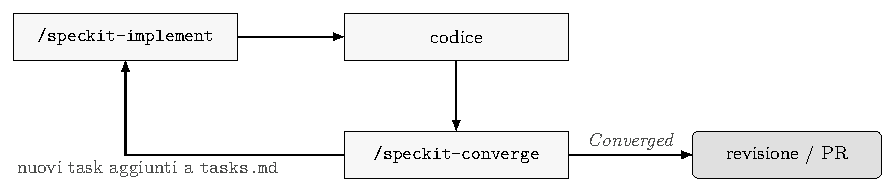
\includegraphics[keepaspectratio,alt={Il ciclo
implement--converge}]{figure/ciclo-implement-converge.pdf}}
\caption{Il ciclo implement--converge}
\end{figure}

Quando converge riporta \texttt{Converged}, il lavoro è completo: puoi
procedere con la revisione umana o aprire la pull request.

\subsection{3.13.5 Cosa garantisce la
convergenza}\label{cosa-garantisce-la-convergenza}

La convergenza è ciò che trasforma ``l'agente ha scritto del codice'' in
``l'agente ha scritto \textbf{il} codice richiesto''. È una verifica di
\textbf{completezza}, non di correttezza: i test (scritti in modalità
test-first) coprono la correttezza; la convergenza copre la completezza.
Insieme, danno una ragionevole fiducia che il risultato corrisponda alla
specifica.

\subsection{3.13.6 Il risultato finale}\label{il-risultato-finale}

Al termine del flusso completo hai:

\begin{itemize}
\tightlist
\item
  una specifica rivista (\texttt{spec.md});
\item
  un piano tecnico con modello dati e contratti;
\item
  una lista di task eseguiti;
\item
  il codice sorgente;
\item
  i test;
\item
  la conferma di convergenza.
\end{itemize}

E tutto è \textbf{versionato}: chiunque riapra la feature --- un
collega, un revisore, o te stesso tra sei mesi --- trova non solo il
codice, ma il \emph{perché} e il \emph{come} documentati.

\section{\texorpdfstring{3.14 Il CLI
\texttt{specify}}{3.14 Il CLI specify}}\label{il-cli-specify}

I comandi \texttt{/speckit-*} vivono nella chat dell'agente, ma Spec Kit
include anche un \textbf{CLI} (\texttt{specify}) per le operazioni di
terra: inizializzazione, controlli dei prerequisiti, gestione di
estensioni, preset e workflow.

\subsection{3.14.1 I comandi principali}\label{i-comandi-principali}

{\def\LTcaptype{none} % do not increment counter
\begin{longtable}[]{@{}
  >{\raggedright\arraybackslash}p{(\linewidth - 2\tabcolsep) * \real{0.5625}}
  >{\raggedright\arraybackslash}p{(\linewidth - 2\tabcolsep) * \real{0.4375}}@{}}
\toprule\noalign{}
\begin{minipage}[b]{\linewidth}\raggedright
Comando
\end{minipage} & \begin{minipage}[b]{\linewidth}\raggedright
Scopo
\end{minipage} \\
\midrule\noalign{}
\endhead
\bottomrule\noalign{}
\endlastfoot
\texttt{specify\ init} & Inizializza un progetto (già visto) \\
\texttt{specify\ check} & Controlla la disponibilità degli strumenti e
dei prerequisiti CLI \\
\texttt{specify\ extension\ add\ \textless{}nome\textgreater{}} &
Installa un'estensione (per esempio \texttt{bug}, \texttt{assess}) \\
\texttt{specify\ preset\ search/apply} & Cerca e applica preset della
comunità \\
\texttt{specify\ workflow\ search/run} & Cerca ed esegue workflow \\
\texttt{specify\ bundle\ search/install} & Cerca e installa bundle \\
\end{longtable}
}

\subsection{\texorpdfstring{3.14.2
\texttt{specify\ check}}{3.14.2 specify check}}\label{specify-check}

Il comando \texttt{specify\ check} controlla la disponibilità degli
strumenti e dei prerequisiti richiesti dal CLI nella versione
installata. Non legge né convalida la coerenza di \texttt{spec.md},
\texttt{plan.md}, \texttt{tasks.md} o degli altri artefatti; per questi
servono la revisione e i controlli del workflow Spec Kit (per esempio
\texttt{/speckit-analyze} e \texttt{/speckit-converge}).

\begin{Shaded}
\begin{Highlighting}[]
\ExtensionTok{specify}\NormalTok{ check}
\end{Highlighting}
\end{Shaded}

Se manca un prerequisito, il comando segnala il problema e può
restituire un codice di uscita diverso da zero.
\texttt{specify\ self\ check}, se disponibile nella versione installata,
è un'autodiagnosi del CLI; non è un validatore degli artefatti del
progetto.

\subsection{3.14.3 Le estensioni: bug fixing e
assessment}\label{le-estensioni-bug-fixing-e-assessment}

Abbiamo accennato ai due processi opzionali. Si installano come
estensioni:

\begin{Shaded}
\begin{Highlighting}[]
\ExtensionTok{specify}\NormalTok{ extension add bug}
\ExtensionTok{specify}\NormalTok{ extension add assess}
\end{Highlighting}
\end{Shaded}

\textbf{Bug fixing} aggiunge i comandi:

\begin{Shaded}
\begin{Highlighting}[]
\NormalTok{/speckit{-}bug{-}assess "Sottomettere una password vuota manda in crash il form." slug=login{-}crash}
\NormalTok{/speckit{-}bug{-}fix slug=login{-}crash}
\NormalTok{/speckit{-}bug{-}test slug=login{-}crash}
\end{Highlighting}
\end{Shaded}

Gli artefatti finiscono in
\texttt{.specify/bugs/\textless{}slug\textgreater{}/}, e il verdetto
finale è \texttt{verified}, \texttt{partial} o \texttt{failed}: solo
\texttt{verified} conferma la correzione.

\textbf{Idea assessment} aggiunge i comandi:

\begin{Shaded}
\begin{Highlighting}[]
\NormalTok{/speckit{-}assess{-}intake "Consenti agli utenti di lavorare offline." slug=offline{-}mode}
\NormalTok{/speckit{-}assess{-}research slug=offline{-}mode}
\NormalTok{/speckit{-}assess{-}define slug=offline{-}mode}
\NormalTok{/speckit{-}assess{-}shape slug=offline{-}mode}
\NormalTok{/speckit{-}assess{-}decide slug=offline{-}mode}
\end{Highlighting}
\end{Shaded}

Gli artefatti finiscono in
\texttt{.specify/assessments/\textless{}slug\textgreater{}/}, e la
decisione finale è \texttt{go}, \texttt{needs-clarification} o
\texttt{kill}. Se l'idea ottiene un \texttt{go}, il riepilogo di
\texttt{decision.md} diventa l'input di \texttt{/speckit-specify}.

\subsection{3.14.4 Preset e workflow}\label{preset-e-workflow}

\begin{itemize}
\tightlist
\item
  Un \textbf{preset} adatta template, comandi e terminologia agli
  standard del tuo team (per esempio ``richiedi tracciabilità normativa
  nei piani'').
\item
  Un \textbf{workflow} automatizza sequenze di prompt, comandi, gate e
  task di shell: per esempio, un workflow CI che compila ed esegue i
  test del progetto. \texttt{specify\ check} può servire durante la
  configurazione dell'ambiente, ma non è un gate di qualità degli
  artefatti.
\item
  Un \textbf{bundle} impacchetta estensioni, preset e workflow per
  distribuirli a un team o a un ruolo.
\end{itemize}

\subsection{3.14.5 Estensioni e hook}\label{estensioni-e-hook}

Il file \texttt{.specify/extensions.yml} può registrare \textbf{hook},
cioè azioni da eseguire prima o dopo i comandi. Un caso tipico: un hook
\texttt{before\_specify} che crea (o cambia) il \textbf{branch Git}
all'avvio di una feature. Questo è ciò che permette di integrare Spec
Kit con le abitudini del team (feature branch numerati,
\texttt{001-task-manager}, ecc.), senza che il flusso ne dipenda: come
abbiamo visto, la feature attiva è determinata da
\texttt{.specify/feature.json}, non dal branch.

\subsection{3.14.6 Quando usare il CLI}\label{quando-usare-il-cli}

\begin{itemize}
\tightlist
\item
  \texttt{init} --- una volta per progetto;
\item
  \texttt{check} --- per diagnosticare la disponibilità dei
  prerequisiti, non per convalidare gli artefatti;
\item
  \texttt{extension\ add} --- quando attivi un processo opzionale;
\item
  \texttt{preset}/\texttt{workflow}/\texttt{bundle} --- quando adatti
  Spec Kit al tuo team.
\end{itemize}

Il resto del lavoro quotidiano avviene nella chat dell'agente, con i
comandi \texttt{/speckit-*}.

\section{3.15 Esempio C\#: entità, DbContext e
DTO}\label{esempio-c-entituxe0-dbcontext-e-dto}

È il momento di vedere il codice che \texttt{/speckit-implement} produce
seguendo il piano. Partiamo dalle fondamenta: l'entità, il contesto EF
Core e i DTO. Corrispondono ai task \texttt{T003}, \texttt{T004} e
\texttt{T005} della fase ``Foundational''.

\subsection{\texorpdfstring{3.15.1 L'entità
\texttt{TaskItem}}{3.15.1 L'entità TaskItem}}\label{lentituxe0-taskitem}

File \texttt{src/Models/TaskItem.cs}, come stabilito dal piano:

\begin{Shaded}
\begin{Highlighting}[]
\KeywordTok{namespace}\NormalTok{ Taskify}\OperatorTok{.}\FunctionTok{Models}\OperatorTok{;}

\KeywordTok{public} \KeywordTok{sealed} \KeywordTok{class}\NormalTok{ TaskItem}
\OperatorTok{\{}
    \KeywordTok{public} \DataTypeTok{int}\NormalTok{ Id }\OperatorTok{\{} \KeywordTok{get}\OperatorTok{;} \KeywordTok{set}\OperatorTok{;} \OperatorTok{\}}
    \KeywordTok{public}\NormalTok{ required }\DataTypeTok{string}\NormalTok{ Title }\OperatorTok{\{} \KeywordTok{get}\OperatorTok{;} \KeywordTok{set}\OperatorTok{;} \OperatorTok{\}}
    \KeywordTok{public} \DataTypeTok{bool}\NormalTok{ IsCompleted }\OperatorTok{\{} \KeywordTok{get}\OperatorTok{;} \KeywordTok{set}\OperatorTok{;} \OperatorTok{\}}
    \KeywordTok{public}\NormalTok{ DateTime}\OperatorTok{?}\NormalTok{ DueDate }\OperatorTok{\{} \KeywordTok{get}\OperatorTok{;} \KeywordTok{set}\OperatorTok{;} \OperatorTok{\}}
    \KeywordTok{public}\NormalTok{ DateTimeOffset CreatedAt }\OperatorTok{\{} \KeywordTok{get}\OperatorTok{;} \KeywordTok{set}\OperatorTok{;} \OperatorTok{\}}
\OperatorTok{\}}
\end{Highlighting}
\end{Shaded}

È il riflesso diretto del modello dati definito in
\texttt{data-model.md}: un identificativo, un titolo obbligatorio, lo
stato, la scadenza opzionale e la data di creazione. Nessuna sorpresa:
l'entità \textbf{è} il modello dati, tradotto in C\#.

\subsection{\texorpdfstring{3.15.2 Il
\texttt{DbContext}}{3.15.2 Il DbContext}}\label{il-dbcontext}

File \texttt{src/Data/TaskDbContext.cs}:

\begin{Shaded}
\begin{Highlighting}[]
\KeywordTok{using}\NormalTok{ Microsoft}\OperatorTok{.}\FunctionTok{EntityFrameworkCore}\OperatorTok{;}
\KeywordTok{using}\NormalTok{ Taskify}\OperatorTok{.}\FunctionTok{Models}\OperatorTok{;}

\KeywordTok{namespace}\NormalTok{ Taskify}\OperatorTok{.}\FunctionTok{Data}\OperatorTok{;}

\KeywordTok{public} \KeywordTok{sealed} \KeywordTok{class} \FunctionTok{TaskDbContext}\OperatorTok{(}\NormalTok{DbContextOptions}\OperatorTok{\textless{}}\NormalTok{TaskDbContext}\OperatorTok{\textgreater{}}\NormalTok{ options}\OperatorTok{)}
    \OperatorTok{:} \FunctionTok{DbContext}\OperatorTok{(}\NormalTok{options}\OperatorTok{)}
\OperatorTok{\{}
    \KeywordTok{public}\NormalTok{ DbSet}\OperatorTok{\textless{}}\NormalTok{TaskItem}\OperatorTok{\textgreater{}}\NormalTok{ Tasks }\OperatorTok{=\textgreater{}}\NormalTok{ Set}\OperatorTok{\textless{}}\NormalTok{TaskItem}\OperatorTok{\textgreater{}();}

    \KeywordTok{protected} \KeywordTok{override} \DataTypeTok{void} \FunctionTok{OnModelCreating}\OperatorTok{(}\NormalTok{ModelBuilder modelBuilder}\OperatorTok{)}
    \OperatorTok{\{}
\NormalTok{        modelBuilder}\OperatorTok{.}\FunctionTok{Entity}\OperatorTok{\textless{}}\NormalTok{TaskItem}\OperatorTok{\textgreater{}(}\NormalTok{entity }\OperatorTok{=\textgreater{}}
        \OperatorTok{\{}
\NormalTok{            entity}\OperatorTok{.}\FunctionTok{Property}\OperatorTok{(}\NormalTok{t }\OperatorTok{=\textgreater{}}\NormalTok{ t}\OperatorTok{.}\FunctionTok{Title}\OperatorTok{).}\FunctionTok{HasMaxLength}\OperatorTok{(}\DecValTok{200}\OperatorTok{).}\FunctionTok{IsRequired}\OperatorTok{();}
\NormalTok{            entity}\OperatorTok{.}\FunctionTok{Property}\OperatorTok{(}\NormalTok{t }\OperatorTok{=\textgreater{}}\NormalTok{ t}\OperatorTok{.}\FunctionTok{IsCompleted}\OperatorTok{).}\FunctionTok{HasDefaultValue}\OperatorTok{(}\KeywordTok{false}\OperatorTok{);}
        \OperatorTok{\});}
    \OperatorTok{\}}
\OperatorTok{\}}
\end{Highlighting}
\end{Shaded}

Due scelte qui derivano \textbf{direttamente dalla specifica}:

\begin{itemize}
\tightlist
\item
  \texttt{HasMaxLength(200)} --- il vincolo ``titolo massimo 200
  caratteri'' (FR-001) non vive solo nella validazione dell'endpoint, ma
  anche nello schema del database: difesa in profondità;
\item
  \texttt{HasDefaultValue(false)} --- un task nasce ``aperto''.
\end{itemize}

\subsection{3.15.3 I DTO}\label{i-dto}

File \texttt{src/Contracts/TaskDtos.cs}:

\begin{Shaded}
\begin{Highlighting}[]
\KeywordTok{using}\NormalTok{ Taskify}\OperatorTok{.}\FunctionTok{Models}\OperatorTok{;}

\KeywordTok{namespace}\NormalTok{ Taskify}\OperatorTok{.}\FunctionTok{Contracts}\OperatorTok{;}

\KeywordTok{public} \KeywordTok{sealed}\NormalTok{ record }\FunctionTok{CreateTaskRequest}\OperatorTok{(}\DataTypeTok{string}\OperatorTok{?}\NormalTok{ Title}\OperatorTok{,}\NormalTok{ DateTime}\OperatorTok{?}\NormalTok{ DueDate}\OperatorTok{);}

\KeywordTok{public} \KeywordTok{sealed}\NormalTok{ record }\FunctionTok{TaskDto}\OperatorTok{(}
    \DataTypeTok{int}\NormalTok{ Id}\OperatorTok{,}
    \DataTypeTok{string}\NormalTok{ Title}\OperatorTok{,}
    \DataTypeTok{bool}\NormalTok{ IsCompleted}\OperatorTok{,}
\NormalTok{    DateTime}\OperatorTok{?}\NormalTok{ DueDate}\OperatorTok{,}
\NormalTok{    DateTimeOffset CreatedAt}\OperatorTok{)}
\OperatorTok{\{}
    \KeywordTok{public} \KeywordTok{static}\NormalTok{ TaskDto }\FunctionTok{From}\OperatorTok{(}\NormalTok{TaskItem task}\OperatorTok{)} \OperatorTok{=\textgreater{}} \KeywordTok{new}\OperatorTok{(}
\NormalTok{        task}\OperatorTok{.}\FunctionTok{Id}\OperatorTok{,}
\NormalTok{        task}\OperatorTok{.}\FunctionTok{Title}\OperatorTok{,}
\NormalTok{        task}\OperatorTok{.}\FunctionTok{IsCompleted}\OperatorTok{,}
\NormalTok{        task}\OperatorTok{.}\FunctionTok{DueDate}\OperatorTok{,}
\NormalTok{        task}\OperatorTok{.}\FunctionTok{CreatedAt}\OperatorTok{);}
\OperatorTok{\}}
\end{Highlighting}
\end{Shaded}

Il DTO separa il \textbf{contratto esterno} (ciò che l'API espone) dal
\textbf{modello interno} (l'entità EF Core). È la pratica del Capitolo 2
applicata qui: mai esporre le entità grezze, controllare sempre ciò che
viaggia sul filo.

\subsection{3.15.4 La tracciabilità spec →
codice}\label{la-tracciabilituxe0-spec-codice}

Nota come ogni decisione di codice sia riconducibile a un requisito:

{\def\LTcaptype{none} % do not increment counter
\begin{longtable}[]{@{}ll@{}}
\toprule\noalign{}
Codice & Requisito di origine \\
\midrule\noalign{}
\endhead
\bottomrule\noalign{}
\endlastfoot
\texttt{Title} obbligatorio, max 200 & FR-001 \\
\texttt{IsCompleted} con default \texttt{false} & FR-003
(completamento) \\
\texttt{DueDate?} opzionale & FR-001 \\
\texttt{TaskDto.From} (proiezione) & Coerenza API (constitution) \\
\end{longtable}
}

Questa tracciabilità non è un vezzo: è ciò che permette, durante la
\textbf{convergenza}, di verificare che ogni requisito abbia una
realizzazione nel codice.

\subsection{3.15.5 La registrazione dei
servizi}\label{la-registrazione-dei-servizi}

L'ultimo tassello ``foundational'' è la registrazione del
\texttt{DbContext} nel container (task \texttt{T006}), che vedremo
all'inizio di \texttt{Program.cs} nella prossima sezione. Con queste
fondamenta pronte, il ``Checkpoint'' della fase Foundational è superato:
le user story possono essere implementate.

\section{3.16 Esempio C\#: gli endpoint della Minimal
API}\label{esempio-c-gli-endpoint-della-minimal-api}

Ecco il cuore dell'implementazione: \texttt{src/Program.cs}, che
realizza i quattro endpoint definiti nei contratti. Il listato mostra lo
stato finale del file dopo il ciclo test-first; corrisponde ai task di
implementazione \texttt{T009}, \texttt{T013} e \texttt{T017}. L'ordine
espositivo del capitolo non è l'ordine di lavoro: i test vanno scritti
ed eseguiti in RED prima di implementare gli endpoint.

\subsection{3.16.1 Il codice completo}\label{il-codice-completo}

\begin{Shaded}
\begin{Highlighting}[]
\KeywordTok{using}\NormalTok{ Microsoft}\OperatorTok{.}\FunctionTok{EntityFrameworkCore}\OperatorTok{;}
\KeywordTok{using}\NormalTok{ Taskify}\OperatorTok{.}\FunctionTok{Contracts}\OperatorTok{;}
\KeywordTok{using}\NormalTok{ Taskify}\OperatorTok{.}\FunctionTok{Data}\OperatorTok{;}
\KeywordTok{using}\NormalTok{ Taskify}\OperatorTok{.}\FunctionTok{Models}\OperatorTok{;}

\DataTypeTok{var}\NormalTok{ builder }\OperatorTok{=}\NormalTok{ WebApplication}\OperatorTok{.}\FunctionTok{CreateBuilder}\OperatorTok{(}\NormalTok{args}\OperatorTok{);}

\NormalTok{builder}\OperatorTok{.}\FunctionTok{Services}\OperatorTok{.}\FunctionTok{AddDbContext}\OperatorTok{\textless{}}\NormalTok{TaskDbContext}\OperatorTok{\textgreater{}(}\NormalTok{options }\OperatorTok{=\textgreater{}}
\NormalTok{    options}\OperatorTok{.}\FunctionTok{UseSqlite}\OperatorTok{(}\StringTok{"Data Source=tasks.db"}\OperatorTok{));}

\DataTypeTok{var}\NormalTok{ app }\OperatorTok{=}\NormalTok{ builder}\OperatorTok{.}\FunctionTok{Build}\OperatorTok{();}

\CommentTok{// Crea lo schema all\textquotesingle{}avvio (solo per l\textquotesingle{}esempio; in produzione: migrazioni).}
\KeywordTok{using} \OperatorTok{(}\DataTypeTok{var}\NormalTok{ scope }\OperatorTok{=}\NormalTok{ app}\OperatorTok{.}\FunctionTok{Services}\OperatorTok{.}\FunctionTok{CreateScope}\OperatorTok{())}
\OperatorTok{\{}
    \DataTypeTok{var}\NormalTok{ db }\OperatorTok{=}\NormalTok{ scope}\OperatorTok{.}\FunctionTok{ServiceProvider}\OperatorTok{.}\FunctionTok{GetRequiredService}\OperatorTok{\textless{}}\NormalTok{TaskDbContext}\OperatorTok{\textgreater{}();}
\NormalTok{    db}\OperatorTok{.}\FunctionTok{Database}\OperatorTok{.}\FunctionTok{EnsureCreated}\OperatorTok{();}
\OperatorTok{\}}

\CommentTok{// {-}{-}{-}{-} US1: creare un task {-}{-}{-}{-}}
\NormalTok{app}\OperatorTok{.}\FunctionTok{MapPost}\OperatorTok{(}\StringTok{"/tasks"}\OperatorTok{,} \FunctionTok{async} \OperatorTok{(}\NormalTok{CreateTaskRequest request}\OperatorTok{,}\NormalTok{ TaskDbContext db}\OperatorTok{)} \OperatorTok{=\textgreater{}}
\OperatorTok{\{}
    \KeywordTok{if} \OperatorTok{(}\DataTypeTok{string}\OperatorTok{.}\FunctionTok{IsNullOrWhiteSpace}\OperatorTok{(}\NormalTok{request}\OperatorTok{.}\FunctionTok{Title}\OperatorTok{))}
        \KeywordTok{return}\NormalTok{ Results}\OperatorTok{.}\FunctionTok{BadRequest}\OperatorTok{(}\KeywordTok{new} \OperatorTok{\{}\NormalTok{ error }\OperatorTok{=} \StringTok{"Title is required."} \OperatorTok{\});}

    \KeywordTok{if} \OperatorTok{(}\NormalTok{request}\OperatorTok{.}\FunctionTok{Title}\OperatorTok{.}\FunctionTok{Length} \OperatorTok{\textgreater{}} \DecValTok{200}\OperatorTok{)}
        \KeywordTok{return}\NormalTok{ Results}\OperatorTok{.}\FunctionTok{BadRequest}\OperatorTok{(}\KeywordTok{new} \OperatorTok{\{}\NormalTok{ error }\OperatorTok{=} \StringTok{"Title must be at most 200 characters."} \OperatorTok{\});}

    \DataTypeTok{var}\NormalTok{ task }\OperatorTok{=} \KeywordTok{new}\NormalTok{ TaskItem}
    \OperatorTok{\{}
\NormalTok{        Title }\OperatorTok{=}\NormalTok{ request}\OperatorTok{.}\FunctionTok{Title}\OperatorTok{,}
\NormalTok{        DueDate }\OperatorTok{=}\NormalTok{ request}\OperatorTok{.}\FunctionTok{DueDate}\OperatorTok{,}
\NormalTok{        IsCompleted }\OperatorTok{=} \KeywordTok{false}\OperatorTok{,}
\NormalTok{        CreatedAt }\OperatorTok{=}\NormalTok{ DateTimeOffset}\OperatorTok{.}\FunctionTok{UtcNow}
    \OperatorTok{\};}

\NormalTok{    db}\OperatorTok{.}\FunctionTok{Tasks}\OperatorTok{.}\FunctionTok{Add}\OperatorTok{(}\NormalTok{task}\OperatorTok{);}
\NormalTok{    await db}\OperatorTok{.}\FunctionTok{SaveChangesAsync}\OperatorTok{();}

    \KeywordTok{return}\NormalTok{ Results}\OperatorTok{.}\FunctionTok{Created}\OperatorTok{(}\NormalTok{$}\StringTok{"/tasks/\{task.Id\}"}\OperatorTok{,}\NormalTok{ TaskDto}\OperatorTok{.}\FunctionTok{From}\OperatorTok{(}\NormalTok{task}\OperatorTok{));}
\OperatorTok{\});}

\CommentTok{// {-}{-}{-}{-} US2: elencare e filtrare {-}{-}{-}{-}}
\NormalTok{app}\OperatorTok{.}\FunctionTok{MapGet}\OperatorTok{(}\StringTok{"/tasks"}\OperatorTok{,} \FunctionTok{async} \OperatorTok{(}\DataTypeTok{string}\OperatorTok{?}\NormalTok{ status}\OperatorTok{,}\NormalTok{ TaskDbContext db}\OperatorTok{)} \OperatorTok{=\textgreater{}}
\OperatorTok{\{}
\NormalTok{    IQueryable}\OperatorTok{\textless{}}\NormalTok{TaskItem}\OperatorTok{\textgreater{}}\NormalTok{ query }\OperatorTok{=}\NormalTok{ db}\OperatorTok{.}\FunctionTok{Tasks}\OperatorTok{;}

    \KeywordTok{if} \OperatorTok{(}\NormalTok{status }\KeywordTok{is}\NormalTok{ not }\KeywordTok{null}\OperatorTok{)}
    \OperatorTok{\{}
        \DataTypeTok{var}\NormalTok{ completed }\OperatorTok{=}\NormalTok{ status }\KeywordTok{switch}
        \OperatorTok{\{}
            \StringTok{"open"} \OperatorTok{=\textgreater{}} \KeywordTok{false}\OperatorTok{,}
            \StringTok{"completed"} \OperatorTok{=\textgreater{}} \KeywordTok{true}\OperatorTok{,}
\NormalTok{            \_ }\OperatorTok{=\textgreater{}} \OperatorTok{(}\DataTypeTok{bool}\OperatorTok{?)}\KeywordTok{null}
        \OperatorTok{\};}

        \KeywordTok{if} \OperatorTok{(}\NormalTok{completed }\KeywordTok{is} \KeywordTok{null}\OperatorTok{)}
            \KeywordTok{return}\NormalTok{ Results}\OperatorTok{.}\FunctionTok{BadRequest}\OperatorTok{(}\KeywordTok{new} \OperatorTok{\{}\NormalTok{ error }\OperatorTok{=} \StringTok{"status must be \textquotesingle{}open\textquotesingle{} or \textquotesingle{}completed\textquotesingle{}."} \OperatorTok{\});}

\NormalTok{        query }\OperatorTok{=}\NormalTok{ query}\OperatorTok{.}\FunctionTok{Where}\OperatorTok{(}\NormalTok{t }\OperatorTok{=\textgreater{}}\NormalTok{ t}\OperatorTok{.}\FunctionTok{IsCompleted} \OperatorTok{==}\NormalTok{ completed}\OperatorTok{);}
    \OperatorTok{\}}

    \DataTypeTok{var}\NormalTok{ tasks }\OperatorTok{=}\NormalTok{ await query}
        \OperatorTok{.}\FunctionTok{OrderBy}\OperatorTok{(}\NormalTok{t }\OperatorTok{=\textgreater{}}\NormalTok{ t}\OperatorTok{.}\FunctionTok{Id}\OperatorTok{)}
        \OperatorTok{.}\FunctionTok{Select}\OperatorTok{(}\NormalTok{t }\OperatorTok{=\textgreater{}} \KeywordTok{new} \FunctionTok{TaskDto}\OperatorTok{(}
\NormalTok{            t}\OperatorTok{.}\FunctionTok{Id}\OperatorTok{,}
\NormalTok{            t}\OperatorTok{.}\FunctionTok{Title}\OperatorTok{,}
\NormalTok{            t}\OperatorTok{.}\FunctionTok{IsCompleted}\OperatorTok{,}
\NormalTok{            t}\OperatorTok{.}\FunctionTok{DueDate}\OperatorTok{,}
\NormalTok{            t}\OperatorTok{.}\FunctionTok{CreatedAt}\OperatorTok{))}
        \OperatorTok{.}\FunctionTok{ToListAsync}\OperatorTok{();}

    \KeywordTok{return}\NormalTok{ Results}\OperatorTok{.}\FunctionTok{Ok}\OperatorTok{(}\NormalTok{tasks}\OperatorTok{);}
\OperatorTok{\});}

\CommentTok{// {-}{-}{-}{-} US3: completare {-}{-}{-}{-}}
\NormalTok{app}\OperatorTok{.}\FunctionTok{MapPost}\OperatorTok{(}\StringTok{"/tasks/\{id:int\}/complete"}\OperatorTok{,} \FunctionTok{async} \OperatorTok{(}\DataTypeTok{int}\NormalTok{ id}\OperatorTok{,}\NormalTok{ TaskDbContext db}\OperatorTok{)} \OperatorTok{=\textgreater{}}
\OperatorTok{\{}
    \DataTypeTok{var}\NormalTok{ task }\OperatorTok{=}\NormalTok{ await db}\OperatorTok{.}\FunctionTok{Tasks}\OperatorTok{.}\FunctionTok{FindAsync}\OperatorTok{(}\NormalTok{id}\OperatorTok{);}
    \KeywordTok{if} \OperatorTok{(}\NormalTok{task }\KeywordTok{is} \KeywordTok{null}\OperatorTok{)}
        \KeywordTok{return}\NormalTok{ Results}\OperatorTok{.}\FunctionTok{NotFound}\OperatorTok{(}\KeywordTok{new} \OperatorTok{\{}\NormalTok{ error }\OperatorTok{=} \StringTok{"Task not found."} \OperatorTok{\});}

\NormalTok{    task}\OperatorTok{.}\FunctionTok{IsCompleted} \OperatorTok{=} \KeywordTok{true}\OperatorTok{;}
\NormalTok{    await db}\OperatorTok{.}\FunctionTok{SaveChangesAsync}\OperatorTok{();}

    \KeywordTok{return}\NormalTok{ Results}\OperatorTok{.}\FunctionTok{Ok}\OperatorTok{(}\NormalTok{TaskDto}\OperatorTok{.}\FunctionTok{From}\OperatorTok{(}\NormalTok{task}\OperatorTok{));}
\OperatorTok{\});}

\CommentTok{// {-}{-}{-}{-} US3: eliminare {-}{-}{-}{-}}
\NormalTok{app}\OperatorTok{.}\FunctionTok{MapDelete}\OperatorTok{(}\StringTok{"/tasks/\{id:int\}"}\OperatorTok{,} \FunctionTok{async} \OperatorTok{(}\DataTypeTok{int}\NormalTok{ id}\OperatorTok{,}\NormalTok{ TaskDbContext db}\OperatorTok{)} \OperatorTok{=\textgreater{}}
\OperatorTok{\{}
    \DataTypeTok{var}\NormalTok{ task }\OperatorTok{=}\NormalTok{ await db}\OperatorTok{.}\FunctionTok{Tasks}\OperatorTok{.}\FunctionTok{FindAsync}\OperatorTok{(}\NormalTok{id}\OperatorTok{);}
    \KeywordTok{if} \OperatorTok{(}\NormalTok{task }\KeywordTok{is} \KeywordTok{null}\OperatorTok{)}
        \KeywordTok{return}\NormalTok{ Results}\OperatorTok{.}\FunctionTok{NotFound}\OperatorTok{(}\KeywordTok{new} \OperatorTok{\{}\NormalTok{ error }\OperatorTok{=} \StringTok{"Task not found."} \OperatorTok{\});}

\NormalTok{    db}\OperatorTok{.}\FunctionTok{Tasks}\OperatorTok{.}\FunctionTok{Remove}\OperatorTok{(}\NormalTok{task}\OperatorTok{);}
\NormalTok{    await db}\OperatorTok{.}\FunctionTok{SaveChangesAsync}\OperatorTok{();}

    \KeywordTok{return}\NormalTok{ Results}\OperatorTok{.}\FunctionTok{NoContent}\OperatorTok{();}
\OperatorTok{\});}

\NormalTok{app}\OperatorTok{.}\FunctionTok{Run}\OperatorTok{();}

\CommentTok{// Rende Program accessibile ai test di integrazione (WebApplicationFactory).}
\KeywordTok{public} \KeywordTok{partial} \KeywordTok{class}\NormalTok{ Program }\OperatorTok{\{} \OperatorTok{\}}
\end{Highlighting}
\end{Shaded}

\subsection{3.16.2 Lettura guidata}\label{lettura-guidata}

\textbf{La Minimal API.} Abbiamo scelto il pattern \emph{Minimal API} di
ASP.NET Core: endpoint dichiarati con \texttt{MapPost}, \texttt{MapGet},
\texttt{MapDelete}, handler come lambda. È la scelta più
\textbf{semplice} per una feature di questo calibro --- coerente con il
principio di Semplicità della constitution. Se la feature crescesse, il
piano potrebbe evolvere verso i controller; per ora, minimal è la scelta
giusta.

\textbf{La validazione.} I due controlli su \texttt{Title}
(obbligatorietà e lunghezza) realizzano FR-001 e il principio di
Validazione della constitution. Errori chiari
(\texttt{Title\ is\ required.}) permettono al chiamante di correggersi.

\textbf{I codici di stato.} Ogni risposta usa un codice semantico:
\texttt{201\ Created} con l'URI della risorsa,
\texttt{400\ Bad\ Request} per input non validi,
\texttt{404\ Not\ Found} per risorse inesistenti,
\texttt{204\ No\ Content} per l'eliminazione. È la coerenza REST
richiesta dalla constitution.

\textbf{Il binding dei parametri.} ASP.NET Core associa automaticamente
il corpo JSON a \texttt{CreateTaskRequest}, i segmenti di route a
\texttt{id}, la query string a \texttt{status}, e inietta il
\texttt{TaskDbContext} dall'DI. Nessun codice di colla.

\textbf{\texttt{public\ partial\ class\ Program}.} L'ultima riga rende
la classe \texttt{Program} (generata dai top-level statements)
accessibile al progetto di test, che userà
\texttt{WebApplicationFactory\textless{}Program\textgreater{}}. È un
dettaglio indispensabile per i test di integrazione.

\subsection{3.16.3 Il progetto}\label{il-progetto}

Il progetto web si crea con:

\begin{Shaded}
\begin{Highlighting}[]
\OperatorTok{\textgreater{}}\NormalTok{ dotnet }\ExtensionTok{new}\NormalTok{ web }\AttributeTok{{-}o}\NormalTok{ src }\AttributeTok{{-}n}\NormalTok{ Taskify}
\OperatorTok{\textgreater{}}\NormalTok{ cd }\ExtensionTok{src}
\OperatorTok{\textgreater{}}\NormalTok{ dotnet }\ExtensionTok{add}\NormalTok{ package Microsoft.EntityFrameworkCore.Sqlite}
\end{Highlighting}
\end{Shaded}

Il file di progetto usa \texttt{Microsoft.NET.Sdk.Web}, che include
implicitamente i namespaces di ASP.NET Core (per questo nel listato non
servono molti \texttt{using} espliciti).

\section{3.17 Esempio C\#: i test
(test-first)}\label{esempio-c-i-test-test-first}

La constitution impone il \textbf{Test-First}, e i task lo riflettono:
prima i test, poi l'implementazione. Il listato mostra il file completo
a lavoro terminato; durante il lavoro si aggiungono i test di ciascuna
user story e li si esegue in RED prima di implementare la story
corrispondente.

\subsection{3.17.1 Il progetto di test}\label{il-progetto-di-test}

\begin{Shaded}
\begin{Highlighting}[]
\OperatorTok{\textgreater{}}\NormalTok{ dotnet }\ExtensionTok{new}\NormalTok{ xunit }\AttributeTok{{-}o}\NormalTok{ tests/Taskify.Tests }\AttributeTok{{-}n}\NormalTok{ Taskify.Tests}
\OperatorTok{\textgreater{}}\NormalTok{ dotnet }\ExtensionTok{add}\NormalTok{ tests/Taskify.Tests/Taskify.Tests.csproj reference src/Taskify.csproj}
\OperatorTok{\textgreater{}}\NormalTok{ dotnet }\ExtensionTok{add}\NormalTok{ tests/Taskify.Tests/Taskify.Tests.csproj package Microsoft.AspNetCore.Mvc.Testing}
\end{Highlighting}
\end{Shaded}

Il pacchetto \texttt{Microsoft.AspNetCore.Mvc.Testing} fornisce
\texttt{WebApplicationFactory\textless{}T\textgreater{}}, che avvia
l'applicazione \textbf{in-memory} per i test di integrazione, senza
bisogno di un server reale.

\subsection{3.17.2 I test}\label{i-test}

File \texttt{tests/Taskify.Tests/TaskEndpointsTests.cs}:

\begin{Shaded}
\begin{Highlighting}[]
\KeywordTok{using}\NormalTok{ System}\OperatorTok{.}\FunctionTok{Net}\OperatorTok{;}
\KeywordTok{using}\NormalTok{ System}\OperatorTok{.}\FunctionTok{Net}\OperatorTok{.}\FunctionTok{Http}\OperatorTok{.}\FunctionTok{Json}\OperatorTok{;}
\KeywordTok{using}\NormalTok{ Microsoft}\OperatorTok{.}\FunctionTok{AspNetCore}\OperatorTok{.}\FunctionTok{Mvc}\OperatorTok{.}\FunctionTok{Testing}\OperatorTok{;}
\KeywordTok{using}\NormalTok{ Taskify}\OperatorTok{.}\FunctionTok{Contracts}\OperatorTok{;}

\KeywordTok{namespace}\NormalTok{ Taskify}\OperatorTok{.}\FunctionTok{Tests}\OperatorTok{;}

\KeywordTok{public} \KeywordTok{class}\NormalTok{ TaskEndpointsTests }\OperatorTok{:}\NormalTok{ IClassFixture}\OperatorTok{\textless{}}\NormalTok{WebApplicationFactory}\OperatorTok{\textless{}}\NormalTok{Program}\OperatorTok{\textgreater{}\textgreater{}}
\OperatorTok{\{}
    \KeywordTok{private} \KeywordTok{readonly}\NormalTok{ HttpClient \_client}\OperatorTok{;}

    \KeywordTok{public} \FunctionTok{TaskEndpointsTests}\OperatorTok{(}\NormalTok{WebApplicationFactory}\OperatorTok{\textless{}}\NormalTok{Program}\OperatorTok{\textgreater{}}\NormalTok{ factory}\OperatorTok{)}
    \OperatorTok{\{}
\NormalTok{        \_client }\OperatorTok{=}\NormalTok{ factory}\OperatorTok{.}\FunctionTok{CreateClient}\OperatorTok{();}
    \OperatorTok{\}}

    \OperatorTok{[}\NormalTok{Fact}\OperatorTok{]}
    \KeywordTok{public}\NormalTok{ async Task }\FunctionTok{CreateTask\_WithValidTitle\_ReturnsCreated}\OperatorTok{()}
    \OperatorTok{\{}
        \DataTypeTok{var}\NormalTok{ response }\OperatorTok{=}\NormalTok{ await \_client}\OperatorTok{.}\FunctionTok{PostAsJsonAsync}\OperatorTok{(}
            \StringTok{"/tasks"}\OperatorTok{,} \KeywordTok{new} \OperatorTok{\{}\NormalTok{ title }\OperatorTok{=} \StringTok{"Write the tests"}\OperatorTok{,}\NormalTok{ dueDate }\OperatorTok{=} \OperatorTok{(}\NormalTok{DateTime}\OperatorTok{?)}\KeywordTok{null} \OperatorTok{\});}

\NormalTok{        Assert}\OperatorTok{.}\FunctionTok{Equal}\OperatorTok{(}\NormalTok{HttpStatusCode}\OperatorTok{.}\FunctionTok{Created}\OperatorTok{,}\NormalTok{ response}\OperatorTok{.}\FunctionTok{StatusCode}\OperatorTok{);}

        \DataTypeTok{var}\NormalTok{ task }\OperatorTok{=}\NormalTok{ await response}\OperatorTok{.}\FunctionTok{Content}\OperatorTok{.}\FunctionTok{ReadFromJsonAsync}\OperatorTok{\textless{}}\NormalTok{TaskDto}\OperatorTok{\textgreater{}();}
\NormalTok{        Assert}\OperatorTok{.}\FunctionTok{NotNull}\OperatorTok{(}\NormalTok{task}\OperatorTok{);}
\NormalTok{        Assert}\OperatorTok{.}\FunctionTok{Equal}\OperatorTok{(}\StringTok{"Write the tests"}\OperatorTok{,}\NormalTok{ task}\OperatorTok{.}\FunctionTok{Title}\OperatorTok{);}
\NormalTok{        Assert}\OperatorTok{.}\FunctionTok{False}\OperatorTok{(}\NormalTok{task}\OperatorTok{.}\FunctionTok{IsCompleted}\OperatorTok{);}
    \OperatorTok{\}}

    \OperatorTok{[}\NormalTok{Fact}\OperatorTok{]}
    \KeywordTok{public}\NormalTok{ async Task }\FunctionTok{CreateTask\_WithoutTitle\_ReturnsBadRequest}\OperatorTok{()}
    \OperatorTok{\{}
        \DataTypeTok{var}\NormalTok{ response }\OperatorTok{=}\NormalTok{ await \_client}\OperatorTok{.}\FunctionTok{PostAsJsonAsync}\OperatorTok{(}
            \StringTok{"/tasks"}\OperatorTok{,} \KeywordTok{new} \OperatorTok{\{}\NormalTok{ title }\OperatorTok{=} \StringTok{""}\OperatorTok{,}\NormalTok{ dueDate }\OperatorTok{=} \OperatorTok{(}\NormalTok{DateTime}\OperatorTok{?)}\KeywordTok{null} \OperatorTok{\});}

\NormalTok{        Assert}\OperatorTok{.}\FunctionTok{Equal}\OperatorTok{(}\NormalTok{HttpStatusCode}\OperatorTok{.}\FunctionTok{BadRequest}\OperatorTok{,}\NormalTok{ response}\OperatorTok{.}\FunctionTok{StatusCode}\OperatorTok{);}
    \OperatorTok{\}}

    \OperatorTok{[}\NormalTok{Fact}\OperatorTok{]}
    \KeywordTok{public}\NormalTok{ async Task }\FunctionTok{ListTasks\_FilterByStatus\_ReturnsOnlyOpenTasks}\OperatorTok{()}
    \OperatorTok{\{}
\NormalTok{        await \_client}\OperatorTok{.}\FunctionTok{PostAsJsonAsync}\OperatorTok{(}\StringTok{"/tasks"}\OperatorTok{,} \KeywordTok{new} \OperatorTok{\{}\NormalTok{ title }\OperatorTok{=} \StringTok{"Open task"} \OperatorTok{\});}
\NormalTok{        await \_client}\OperatorTok{.}\FunctionTok{PostAsJsonAsync}\OperatorTok{(}\StringTok{"/tasks"}\OperatorTok{,} \KeywordTok{new} \OperatorTok{\{}\NormalTok{ title }\OperatorTok{=} \StringTok{"Done task"} \OperatorTok{\});}

        \DataTypeTok{var}\NormalTok{ open }\OperatorTok{=}\NormalTok{ await \_client}\OperatorTok{.}\FunctionTok{GetFromJsonAsync}\OperatorTok{\textless{}}\NormalTok{List}\OperatorTok{\textless{}}\NormalTok{TaskDto}\OperatorTok{\textgreater{}\textgreater{}(}\StringTok{"/tasks?status=open"}\OperatorTok{);}

\NormalTok{        Assert}\OperatorTok{.}\FunctionTok{NotNull}\OperatorTok{(}\NormalTok{open}\OperatorTok{);}
\NormalTok{        Assert}\OperatorTok{.}\FunctionTok{All}\OperatorTok{(}\NormalTok{open}\OperatorTok{,}\NormalTok{ t }\OperatorTok{=\textgreater{}}\NormalTok{ Assert}\OperatorTok{.}\FunctionTok{False}\OperatorTok{(}\NormalTok{t}\OperatorTok{.}\FunctionTok{IsCompleted}\OperatorTok{));}
    \OperatorTok{\}}

    \OperatorTok{[}\NormalTok{Fact}\OperatorTok{]}
    \KeywordTok{public}\NormalTok{ async Task }\FunctionTok{CompleteTask\_ExistingId\_ReturnsCompleted}\OperatorTok{()}
    \OperatorTok{\{}
        \DataTypeTok{var}\NormalTok{ created }\OperatorTok{=}\NormalTok{ await \_client}\OperatorTok{.}\FunctionTok{PostAsJsonAsync}\OperatorTok{(}\StringTok{"/tasks"}\OperatorTok{,} \KeywordTok{new} \OperatorTok{\{}\NormalTok{ title }\OperatorTok{=} \StringTok{"To complete"} \OperatorTok{\});}
        \DataTypeTok{var}\NormalTok{ task }\OperatorTok{=}\NormalTok{ await created}\OperatorTok{.}\FunctionTok{Content}\OperatorTok{.}\FunctionTok{ReadFromJsonAsync}\OperatorTok{\textless{}}\NormalTok{TaskDto}\OperatorTok{\textgreater{}();}

        \DataTypeTok{var}\NormalTok{ response }\OperatorTok{=}\NormalTok{ await \_client}\OperatorTok{.}\FunctionTok{PostAsync}\OperatorTok{(}\NormalTok{$}\StringTok{"/tasks/\{task!.Id\}/complete"}\OperatorTok{,} \KeywordTok{null}\OperatorTok{);}

\NormalTok{        Assert}\OperatorTok{.}\FunctionTok{Equal}\OperatorTok{(}\NormalTok{HttpStatusCode}\OperatorTok{.}\FunctionTok{OK}\OperatorTok{,}\NormalTok{ response}\OperatorTok{.}\FunctionTok{StatusCode}\OperatorTok{);}
        \DataTypeTok{var}\NormalTok{ completed }\OperatorTok{=}\NormalTok{ await response}\OperatorTok{.}\FunctionTok{Content}\OperatorTok{.}\FunctionTok{ReadFromJsonAsync}\OperatorTok{\textless{}}\NormalTok{TaskDto}\OperatorTok{\textgreater{}();}
\NormalTok{        Assert}\OperatorTok{.}\FunctionTok{True}\OperatorTok{(}\NormalTok{completed}\OperatorTok{!.}\FunctionTok{IsCompleted}\OperatorTok{);}
    \OperatorTok{\}}

    \OperatorTok{[}\NormalTok{Fact}\OperatorTok{]}
    \KeywordTok{public}\NormalTok{ async Task }\FunctionTok{DeleteTask\_ExistingId\_ReturnsNoContent}\OperatorTok{()}
    \OperatorTok{\{}
        \DataTypeTok{var}\NormalTok{ created }\OperatorTok{=}\NormalTok{ await \_client}\OperatorTok{.}\FunctionTok{PostAsJsonAsync}\OperatorTok{(}\StringTok{"/tasks"}\OperatorTok{,} \KeywordTok{new} \OperatorTok{\{}\NormalTok{ title }\OperatorTok{=} \StringTok{"To delete"} \OperatorTok{\});}
        \DataTypeTok{var}\NormalTok{ task }\OperatorTok{=}\NormalTok{ await created}\OperatorTok{.}\FunctionTok{Content}\OperatorTok{.}\FunctionTok{ReadFromJsonAsync}\OperatorTok{\textless{}}\NormalTok{TaskDto}\OperatorTok{\textgreater{}();}

        \DataTypeTok{var}\NormalTok{ response }\OperatorTok{=}\NormalTok{ await \_client}\OperatorTok{.}\FunctionTok{DeleteAsync}\OperatorTok{(}\NormalTok{$}\StringTok{"/tasks/\{task!.Id\}"}\OperatorTok{);}

\NormalTok{        Assert}\OperatorTok{.}\FunctionTok{Equal}\OperatorTok{(}\NormalTok{HttpStatusCode}\OperatorTok{.}\FunctionTok{NoContent}\OperatorTok{,}\NormalTok{ response}\OperatorTok{.}\FunctionTok{StatusCode}\OperatorTok{);}
    \OperatorTok{\}}
\OperatorTok{\}}
\end{Highlighting}
\end{Shaded}

\subsection{3.17.3 La corrispondenza con gli scenari di
accettazione}\label{la-corrispondenza-con-gli-scenari-di-accettazione}

Ogni test mappa uno scenario della specifica:

{\def\LTcaptype{none} % do not increment counter
\begin{longtable}[]{@{}ll@{}}
\toprule\noalign{}
Test & Scenario di accettazione \\
\midrule\noalign{}
\endhead
\bottomrule\noalign{}
\endlastfoot
\texttt{CreateTask\_WithValidTitle\_ReturnsCreated} & US1, scenario 1 \\
\texttt{CreateTask\_WithoutTitle\_ReturnsBadRequest} & US1, scenario
2 \\
\texttt{ListTasks\_FilterByStatus\_...} & US2, scenario 1 \\
\texttt{CompleteTask\_ExistingId\_...} & US3, scenario 1 \\
\texttt{DeleteTask\_ExistingId\_...} & US3, scenario 2 \\
\end{longtable}
}

È la tracciabilità che la convergenza verificherà: ogni requisito
testabile ha il suo test.

\subsection{3.17.4 Il ciclo
Red-Green-Refactor}\label{il-ciclo-red-green-refactor}

Il principio Test-First impone l'ordine: scrivi il test,
\textbf{verifica che fallisca} (perché l'implementazione non c'è
ancora), poi implementa, poi verifica che passi. In un flusso con agente
AI, questo ordine è importante: evita il ``test scritto a posteriori''
che verrebbe tarato sull'implementazione invece che sul requisito.

\subsection{3.17.5 Eseguire i test}\label{eseguire-i-test}

\begin{Shaded}
\begin{Highlighting}[]
\OperatorTok{\textgreater{}}\NormalTok{ dotnet }\BuiltInTok{test}\NormalTok{ tests/Taskify.Tests/Taskify.Tests.csproj}
\end{Highlighting}
\end{Shaded}

Se tutto è in ordine, l'output riporterà i test verdi. È la conferma di
\textbf{correttezza}; la conferma di \textbf{completezza} arriverà con
\texttt{/speckit-converge}.

\section{3.18 Esempio C\#: eseguire, verificare e
convergere}\label{esempio-c-eseguire-verificare-e-convergere}

Chiudiamo l'esempio eseguendo l'applicazione, provandola con richieste
reali e portando a termine la convergenza.

\subsection{3.18.1 Avviare l'applicazione}\label{avviare-lapplicazione}

\begin{Shaded}
\begin{Highlighting}[]
\OperatorTok{\textgreater{}}\NormalTok{ dotnet run }\OperatorTok{{-}{-}}\NormalTok{urls http}\OperatorTok{://}\NormalTok{localhost}\OperatorTok{:}\DecValTok{5080}
\end{Highlighting}
\end{Shaded}

L'applicazione parte su \texttt{http://localhost:5080}. Ora possiamo
provarla con \texttt{curl.exe} da PowerShell:

\subsection{3.18.2 Creare un task}\label{creare-un-task}

\begin{Shaded}
\begin{Highlighting}[]
\OperatorTok{\textgreater{}} \FunctionTok{curl}\OperatorTok{.}\FunctionTok{exe} \OperatorTok{{-}}\NormalTok{X POST }\StringTok{"http://localhost:5080/tasks"}\NormalTok{ \textasciigrave{}}
    \OperatorTok{{-}}\NormalTok{H }\StringTok{"Content{-}Type: application/json"}\NormalTok{ \textasciigrave{}}
    \OperatorTok{{-}}\NormalTok{d }\StringTok{\textquotesingle{}\{"title": "Scrivere il capitolo 3", "dueDate": null\}\textquotesingle{}}
\end{Highlighting}
\end{Shaded}

Risposta attesa (201 Created):

\begin{Shaded}
\begin{Highlighting}[]
\FunctionTok{\{}
  \DataTypeTok{"id"}\FunctionTok{:} \DecValTok{1}\FunctionTok{,}
  \DataTypeTok{"title"}\FunctionTok{:} \StringTok{"Scrivere il capitolo 3"}\FunctionTok{,}
  \DataTypeTok{"isCompleted"}\FunctionTok{:} \KeywordTok{false}\FunctionTok{,}
  \DataTypeTok{"dueDate"}\FunctionTok{:} \KeywordTok{null}\FunctionTok{,}
  \DataTypeTok{"createdAt"}\FunctionTok{:} \StringTok{"2026{-}10{-}27T12:00:00+00:00"}
\FunctionTok{\}}
\end{Highlighting}
\end{Shaded}

\subsection{3.18.3 Elencare con filtro}\label{elencare-con-filtro}

\begin{Shaded}
\begin{Highlighting}[]
\OperatorTok{\textgreater{}} \FunctionTok{curl}\OperatorTok{.}\FunctionTok{exe} \StringTok{"http://localhost:5080/tasks?status=open"}
\end{Highlighting}
\end{Shaded}

\begin{Shaded}
\begin{Highlighting}[]
\OtherTok{[}
  \FunctionTok{\{} \DataTypeTok{"id"}\FunctionTok{:} \DecValTok{1}\FunctionTok{,} \DataTypeTok{"title"}\FunctionTok{:} \StringTok{"Scrivere il capitolo 3"}\FunctionTok{,} \DataTypeTok{"isCompleted"}\FunctionTok{:} \KeywordTok{false}\FunctionTok{,} \ErrorTok{...} \FunctionTok{\}}
\OtherTok{]}
\end{Highlighting}
\end{Shaded}

\subsection{3.18.4 Completare ed
eliminare}\label{completare-ed-eliminare}

\begin{Shaded}
\begin{Highlighting}[]
\OperatorTok{\textgreater{}} \FunctionTok{curl}\OperatorTok{.}\FunctionTok{exe} \OperatorTok{{-}}\NormalTok{X POST }\StringTok{"http://localhost:5080/tasks/1/complete"}
\OperatorTok{\textgreater{}} \FunctionTok{curl}\OperatorTok{.}\FunctionTok{exe} \OperatorTok{{-}}\NormalTok{X DELETE }\StringTok{"http://localhost:5080/tasks/1"}
\end{Highlighting}
\end{Shaded}

La prima risponde con il task completato, la seconda con
\texttt{204\ No\ Content}.

\subsection{3.18.5 La convergenza}\label{la-convergenza}

Apri una nuova shell nella radice del repository e verifica che i test
passino
(\texttt{dotnet\ test\ tests/Taskify.Tests/Taskify.Tests.csproj}); poi
torniamo all'agente e invochiamo:

\begin{Shaded}
\begin{Highlighting}[]
\NormalTok{/speckit{-}converge}
\end{Highlighting}
\end{Shaded}

Il comando confronta il codice con \texttt{spec.md}, \texttt{plan.md} e
\texttt{tasks.md}. Se tutto è implementato, riporta \textbf{Converged}.
Se, per esempio, avessimo dimenticato la validazione della data di
scadenza nel passato (un edge case della specifica), converge lo
segnalerebbe e \textbf{aggiungerebbe un task} a \texttt{tasks.md}: a
quel punto basterebbe rieseguire \texttt{/speckit-implement} e di nuovo
\texttt{/speckit-converge}.

\subsection{3.18.6 Il risultato completo}\label{il-risultato-completo}

Al termine del flusso, il repository contiene:

\begin{figure}
\centering
\pandocbounded{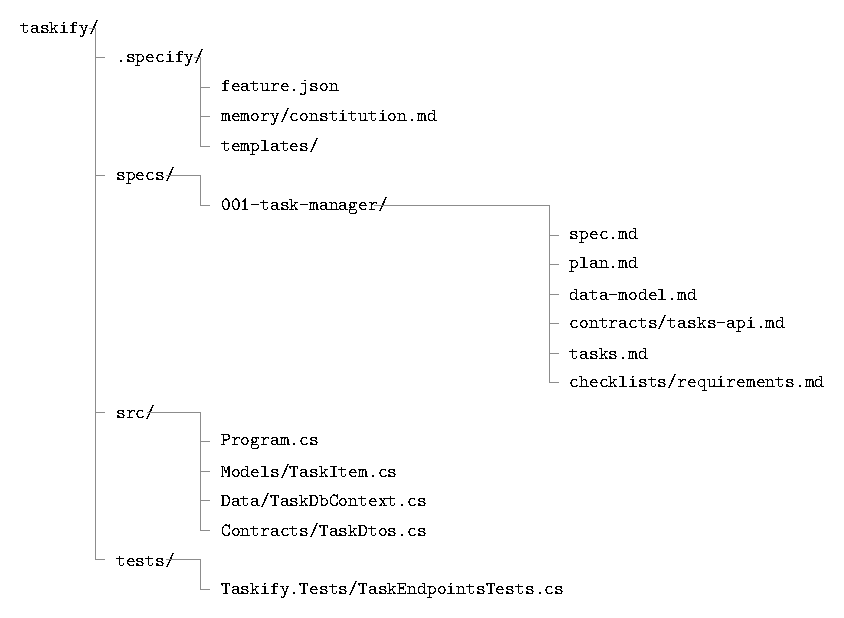
\includegraphics[keepaspectratio,alt={Struttura finale
del repository dopo il flusso completo}]{figure/risultato-finale.pdf}}
\caption{Struttura finale del repository dopo il flusso completo}
\end{figure}

Una feature completa: specifica, piano, task, codice, test e convergenza
--- tutto versionato e ricostruibile. È il percorso che abbiamo
attraversato in questo capitolo, e che puoi ora ripetere per qualsiasi
feature in C\# (o in qualunque altro linguaggio).

\section{3.19 Integrazione con Copilot e VS
Code}\label{integrazione-con-copilot-e-vs-code}

Spec Kit è agente-agnostico, ma la combinazione più naturale per chi
lavora in .NET è \textbf{Visual Studio Code + GitHub Copilot}. Vediamo
come si presenta l'integrazione.

\subsection{3.19.1 L'integrazione Copilot}\label{lintegrazione-copilot}

Quando esegui \texttt{specify\ init\ -\/-integration\ copilot}, Spec Kit
registra i comandi \texttt{/speckit-*} come \textbf{skill di Copilot}
nel progetto. In VS Code, questo significa che nella chat di Copilot (o
nell'editor) puoi digitare:

\begin{Shaded}
\begin{Highlighting}[]
\NormalTok{/speckit{-}specify Crea una Task Manager API con creazione, elenco, completamento ed eliminazione.}
\end{Highlighting}
\end{Shaded}

e Copilot eseguirà il comando, leggendo i template e scrivendo gli
artefatti in \texttt{specs/}.

\subsection{3.19.2 Dove vivono le skill}\label{dove-vivono-le-skill}

A seconda della versione di Copilot, le skill vengono registrate nella
cartella del progetto (per esempio in \texttt{.github/prompts/} o nelle
configurazioni delle skill). Non serve preoccuparsi del dettaglio:
l'importante è che, dopo \texttt{init}, i comandi \texttt{/speckit-*}
siano disponibili nella chat quando il progetto è aperto.

\subsection{3.19.3 Il flusso in VS Code}\label{il-flusso-in-vs-code}

Il ciclo tipico in VS Code:

\begin{enumerate}
\def\labelenumi{\arabic{enumi}.}
\tightlist
\item
  apri il progetto (\texttt{code\ taskify});
\item
  apri la chat di Copilot;
\item
  invochi \texttt{/speckit-specify} con la descrizione;
\item
  \textbf{rileggi} \texttt{spec.md} nell'editor (i file sono lì,
  modificabili a mano);
\item
  invochi i comandi successivi uno alla volta;
\item
  quando arrivi a \texttt{/speckit-implement}, Copilot scrive i file C\#
  nel progetto;
\item
  esegui \texttt{dotnet\ test} nel terminale integrato;
\item
  chiudi con \texttt{/speckit-converge}.
\end{enumerate}

\subsection{3.19.4 Altri agenti}\label{altri-agenti}

Spec Kit supporta molti agenti: Claude Code, Cursor, Windsurf, Qoder,
Amazon Q, Antigravity, Crush, Gemini CLI, Kilo Code, OpenCode, Roo Code
e altri. La sintassi di invocazione cambia leggermente (ogni agente ha
il suo modo di invocare una skill), ma il flusso e gli artefatti sono
identici: è il valore della standardizzazione.

\subsection{3.19.5 Rivedere e modificare a
mano}\label{rivedere-e-modificare-a-mano}

Un punto da non sottovalutare: \textbf{gli artefatti sono file Markdown
normali}. In VS Code puoi aprirli, modificarli, confrontarli con il diff
di Git e rivederli come faresti con qualsiasi documento. Se la specifica
prodotta non ti convince, la correggi a mano e rilanci i comandi
successivi. L'agente è un acceleratore, non un oracolo infallibile.

\subsection{3.19.6 VS Code e Git}\label{vs-code-e-git}

Il flusso Spec Kit si sposa naturalmente con Git: ogni feature ha la sua
cartella in \texttt{specs/}, e (con l'estensione git opzionale) il suo
branch. Commit e pull request diventano i punti di revisione: la
specifica viene rivista e approvata \textbf{prima} che il codice venga
scritto, spostando la review dove costa meno.

\section{3.20 CI/CD e automazione}\label{cicd-e-automazione}

Spec Kit non si limita alla chat: la pipeline può automatizzare build e
test del prodotto, mentre la revisione degli artefatti Spec Kit resta
affidata al workflow dell'agente e ai revisori.

\subsection{\texorpdfstring{3.20.1 \texttt{specify\ check} non è un gate
degli
artefatti}{3.20.1 specify check non è un gate degli artefatti}}\label{specify-check-non-uxe8-un-gate-degli-artefatti}

\texttt{specify\ check} controlla la disponibilità degli strumenti e dei
prerequisiti richiesti dal CLI; non convalida specifiche, piani, task o
altri artefatti. È utile durante la configurazione dell'ambiente, ma non
aggiunge un controllo di qualità degli artefatti alla CI. Anche
\texttt{specify\ self\ check}, se disponibile, è un'autodiagnosi del CLI
e non sostituisce la revisione degli artefatti.

Il comando si può eseguire localmente per diagnosticare l'ambiente. Non
lo inseriamo nel workflow CI d'esempio: se fallisce, segnala un problema
di prerequisiti CLI, non un artefatto Spec Kit non valido.

\subsection{3.20.2 Build e test del progetto
.NET}\label{build-e-test-del-progetto-.net}

Il controllo automatico ripetibile del progetto è la build e
l'esecuzione dei test. I comandi puntano esplicitamente al progetto di
test perché l'esempio non presuppone una soluzione \texttt{.sln} nella
radice:

\begin{Shaded}
\begin{Highlighting}[]
\FunctionTok{steps}\KeywordTok{:}
\AttributeTok{  }\KeywordTok{{-} }\FunctionTok{uses}\KeywordTok{:}\AttributeTok{ actions/setup{-}dotnet@v4}
\AttributeTok{    }\FunctionTok{with}\KeywordTok{:}
\AttributeTok{      }\FunctionTok{dotnet{-}version}\KeywordTok{:}\AttributeTok{ }\StringTok{\textquotesingle{}10.0.x\textquotesingle{}}
\AttributeTok{  }\KeywordTok{{-} }\FunctionTok{run}\KeywordTok{:}\AttributeTok{ dotnet restore tests/Taskify.Tests/Taskify.Tests.csproj}
\AttributeTok{  }\KeywordTok{{-} }\FunctionTok{run}\KeywordTok{:}\AttributeTok{ dotnet build tests/Taskify.Tests/Taskify.Tests.csproj {-}{-}no{-}restore}
\AttributeTok{  }\KeywordTok{{-} }\FunctionTok{run}\KeywordTok{:}\AttributeTok{ dotnet test tests/Taskify.Tests/Taskify.Tests.csproj {-}{-}no{-}build {-}{-}no{-}restore}
\end{Highlighting}
\end{Shaded}

Questi passaggi compilano anche il progetto web referenziato e poi
eseguono i test xUnit.

\subsection{3.20.3 Workflow e hook}\label{workflow-e-hook}

Spec Kit offre due meccanismi per andare oltre:

\begin{itemize}
\tightlist
\item
  \textbf{Hook} (in \texttt{.specify/extensions.yml}) --- azioni
  prima/dopo i comandi. Un hook \texttt{before\_specify} può creare il
  branch Git della feature automaticamente.
\item
  \textbf{Workflow} --- sequenze automatizzate di prompt, comandi, gate
  e task di shell, eseguibili anche senza interazione.
\end{itemize}

Per esempio, un workflow può incapsulare la sequenza
\texttt{dotnet\ build} → \texttt{dotnet\ test} → report. È utile per
ambienti in cui l'agente non è disponibile o per esecuzioni notturne;
non certifica, da solo, la qualità della specifica o del piano.

\subsection{3.20.4 L'automazione non sostituisce la
revisione}\label{lautomazione-non-sostituisce-la-revisione}

La CI qui controlla che il codice compili e che i test passino; non
verifica la qualità degli artefatti Spec Kit né che la specifica
rifletta davvero ciò che serve. Per la coerenza degli artefatti si usano
i controlli dell'agente, come \texttt{/speckit-analyze} e
\texttt{/speckit-converge}, insieme alla revisione umana. La pipeline è
una rete di sicurezza per il codice, non un sostituto del giudizio.

\subsection{3.20.5 Un esempio di pipeline
completa}\label{un-esempio-di-pipeline-completa}

\begin{Shaded}
\begin{Highlighting}[]
\FunctionTok{name}\KeywordTok{:}\AttributeTok{ ci}

\FunctionTok{on}\KeywordTok{:}\AttributeTok{ }\KeywordTok{[}\AttributeTok{push}\KeywordTok{,}\AttributeTok{ pull\_request}\KeywordTok{]}

\FunctionTok{jobs}\KeywordTok{:}
\AttributeTok{  }\FunctionTok{build}\KeywordTok{:}
\AttributeTok{    }\FunctionTok{runs{-}on}\KeywordTok{:}\AttributeTok{ ubuntu{-}latest}
\AttributeTok{    }\FunctionTok{steps}\KeywordTok{:}
\AttributeTok{      }\KeywordTok{{-} }\FunctionTok{uses}\KeywordTok{:}\AttributeTok{ actions/checkout@v4}

\AttributeTok{      }\KeywordTok{{-} }\FunctionTok{name}\KeywordTok{:}\AttributeTok{ Setup .NET 10}
\AttributeTok{        }\FunctionTok{uses}\KeywordTok{:}\AttributeTok{ actions/setup{-}dotnet@v4}
\AttributeTok{        }\FunctionTok{with}\KeywordTok{:}
\AttributeTok{          }\FunctionTok{dotnet{-}version}\KeywordTok{:}\AttributeTok{ }\StringTok{\textquotesingle{}10.0.x\textquotesingle{}}

\AttributeTok{      }\KeywordTok{{-} }\FunctionTok{name}\KeywordTok{:}\AttributeTok{ Restore}
\AttributeTok{        }\FunctionTok{run}\KeywordTok{:}\AttributeTok{ dotnet restore tests/Taskify.Tests/Taskify.Tests.csproj}

\AttributeTok{      }\KeywordTok{{-} }\FunctionTok{name}\KeywordTok{:}\AttributeTok{ Build}
\AttributeTok{        }\FunctionTok{run}\KeywordTok{:}\AttributeTok{ dotnet build tests/Taskify.Tests/Taskify.Tests.csproj {-}{-}no{-}restore}

\AttributeTok{      }\KeywordTok{{-} }\FunctionTok{name}\KeywordTok{:}\AttributeTok{ Test}
\AttributeTok{        }\FunctionTok{run}\KeywordTok{:}\AttributeTok{ dotnet test tests/Taskify.Tests/Taskify.Tests.csproj {-}{-}no{-}build {-}{-}no{-}restore}
\end{Highlighting}
\end{Shaded}

Questa pipeline verifica il prodotto .NET senza attribuire a
\texttt{specify\ check} o a un controllo CLI una validazione che non
svolgono. La qualità del metodo e degli artefatti si rivede nel workflow
Spec Kit.

\section{3.22 Il processo di bug
fixing}\label{il-processo-di-bug-fixing}

Spec Kit non serve solo a costruire feature: include un processo
dedicato alla \textbf{diagnosi e riparazione dei bug}. È un'estensione
opzionale, che si installa quando serve.

\subsection{Come si installa}\label{come-si-installa}

\begin{Shaded}
\begin{Highlighting}[]
\ExtensionTok{specify}\NormalTok{ extension add bug}
\end{Highlighting}
\end{Shaded}

L'estensione aggiunge tre comandi all'agente:

\begin{Shaded}
\begin{Highlighting}[]
\NormalTok{/speckit{-}bug{-}assess "Sottomettere una password vuota manda in crash il login." slug=login{-}crash}
\NormalTok{/speckit{-}bug{-}fix slug=login{-}crash}
\NormalTok{/speckit{-}bug{-}test slug=login{-}crash}
\end{Highlighting}
\end{Shaded}

\subsection{Il flusso in tre passi}\label{il-flusso-in-tre-passi}

\begin{enumerate}
\def\labelenumi{\arabic{enumi}.}
\tightlist
\item
  \textbf{Assess} --- analizza il sintomo, ne individua la causa
  probabile e delimita l'ambito della correzione. Produce un report in
  \texttt{.specify/bugs/\textless{}slug\textgreater{}/}.
\item
  \textbf{Fix} --- applica la correzione mirata, senza riscrivere interi
  moduli.
\item
  \textbf{Test} --- verifica che il sintomo originale sia risolto e
  registra l'esito.
\end{enumerate}

\subsection{Il verdetto}\label{il-verdetto}

Il passo finale produce un \textbf{verdetto} documentato:

{\def\LTcaptype{none} % do not increment counter
\begin{longtable}[]{@{}ll@{}}
\toprule\noalign{}
Verdetto & Significato \\
\midrule\noalign{}
\endhead
\bottomrule\noalign{}
\endlastfoot
\texttt{verified} & La correzione risolve il sintomo: successo \\
\texttt{partial} & Il sintomo è attenuato ma non del tutto risolto \\
\texttt{failed} & La correzione non risolve il sintomo \\
\end{longtable}
}

Solo \texttt{verified} conferma una correzione riuscita. Gli artefatti
restano in \texttt{.specify/bugs/\textless{}slug\textgreater{}/} come
\textbf{registrazione verificata} di ciò che è stato fatto: causa
valutata, fix delimitato, verifica documentata.

\subsection{Un esempio in C\#}\label{un-esempio-in-c}

Supponiamo che la nostra Task Manager API abbia un bug: creare un task
con un titolo di esattamente 201 caratteri produce un errore 500 invece
di un 400. Il flusso:

\begin{Shaded}
\begin{Highlighting}[]
\NormalTok{/speckit{-}bug{-}assess "POST /tasks con titolo di 201 caratteri restituisce 500}
\NormalTok{invece di 400." slug=title{-}length{-}500}
\end{Highlighting}
\end{Shaded}

L'assessment individua la causa: la validazione controlla
\texttt{Title.Length\ \textgreater{}\ 200} \textbf{dopo} il salvataggio,
ma il database (vincolo \texttt{HasMaxLength(200)}) lancia un'eccezione
prima che la validazione venga raggiunta, producendo il 500.

\begin{Shaded}
\begin{Highlighting}[]
\NormalTok{/speckit{-}bug{-}fix slug=title{-}length{-}500}
\end{Highlighting}
\end{Shaded}

Il fix sposta la validazione della lunghezza \textbf{prima}
dell'inserimento nel database:

\begin{Shaded}
\begin{Highlighting}[]
\CommentTok{// Prima del fix: la validazione arrivava dopo il database}
\CommentTok{// Dopo il fix: la validazione avviene prima di toccare il DbContext}
\KeywordTok{if} \OperatorTok{(}\NormalTok{request}\OperatorTok{.}\FunctionTok{Title} \KeywordTok{is} \OperatorTok{\{}\NormalTok{ Length}\OperatorTok{:} \OperatorTok{\textgreater{}} \DecValTok{200} \OperatorTok{\})}
    \KeywordTok{return}\NormalTok{ Results}\OperatorTok{.}\FunctionTok{BadRequest}\OperatorTok{(}\KeywordTok{new} \OperatorTok{\{}\NormalTok{ error }\OperatorTok{=} \StringTok{"Title must be at most 200 characters."} \OperatorTok{\});}
\end{Highlighting}
\end{Shaded}

\begin{Shaded}
\begin{Highlighting}[]
\NormalTok{/speckit{-}bug{-}test slug=title{-}length{-}500}
\end{Highlighting}
\end{Shaded}

Il test verifica che un titolo di 201 caratteri produca ora
\texttt{400\ Bad\ Request} e che il sintomo originale sia scomparso. Il
verdetto finale, se tutto regge, è \texttt{verified}.

\subsection{Bug fixing vs feature
workflow}\label{bug-fixing-vs-feature-workflow}

Il processo di bug fixing \textbf{non richiede} il workflow SDD
completo: puoi diagnosticare e riparare un bug senza una specifica di
feature. I due processi convivono: lo SDD per il nuovo, il bug fixing
per il rotto.

\section{3.21 Best practice e
anti-pattern}\label{best-practice-e-anti-pattern}

Come ogni metodo, Spec Kit funziona se usato bene. Raccogliamo le
pratiche che fanno la differenza e gli errori in cui è facile cadere.

\subsection{3.21.1 Le best practice}\label{le-best-practice}

\textbf{Una feature, una specifica, un flusso.} Non accumulare più
funzionalità in una sola specifica. Una specifica focalizzata è più
facile da rivisitare, pianificare e implementare.

\textbf{Constitution prima di tutto.} Definisci la constitution
\textbf{una volta}, con cura, e falla rispettare dai gate. Una
constitution vaga è inutile; una constitution chiara è il tuo ``standard
di qualità'' codificato.

\textbf{Un comando alla volta, con revisione.} Non incatenare i comandi.
Rivedi \texttt{spec.md} prima di pianificare, \texttt{plan.md} prima di
scomporre, \texttt{tasks.md} prima di implementare. Il costo della
revisione cresce con l'avanzamento.

\textbf{Risolvi i \texttt{{[}NEEDS\ CLARIFICATION{]}}.} Non lasciarli
nella specifica sperando che l'agente ``ci arrivi'': usa
\texttt{/speckit-clarify} o correggi a mano. Un requisito ambiguo è un
bug in attesa.

\textbf{Mantieni la specifica libera dalla tecnologia.} Lo stack
appartiene al piano, non alla specifica. Se nella specifica leggi ``usa
.NET'', stai mescolando i livelli: la specifica deve dire \emph{cosa},
il piano \emph{come}.

\textbf{Versiona tutto.} Spec, piano, task e constitution sono parte del
repository. La tracciabilità è il valore principale del metodo: non
buttarla via con i \texttt{.gitignore}.

\textbf{Itera sulla convergenza.} Non accontentarti del primo
\texttt{/speckit-converge} se non riporta \texttt{Converged}. Il ciclo
implement→converge è ciò che garantisce la completezza.

\subsection{3.21.2 Gli anti-pattern}\label{gli-anti-pattern}

\textbf{La specifica ``romanzo''.} Una specifica di 50 pagine di prosa è
tanto inutile quanto l'assenza di specifica. Le sezioni strutturate
(user story, FR, SC) esistono per questo: restare concisi e
verificabili.

\textbf{Saltare i gate.} Ignorare \texttt{/speckit-clarify},
\texttt{/speckit-checklist} o \texttt{/speckit-analyze} ``per fare
prima'' sposta i problemi più avanti, dove costano di più.

\textbf{La constitution ipertrofica.} Dieci principi generici (``il
codice deve essere di qualità'') non aiutano. Pochi principi
\textbf{verificabili} valgono più di molti principi generici.

\textbf{Fidarsi ciecamente dell'agente.} L'agente produce bozze di
qualità, ma le decisioni di prodotto sono tue. Rivedi, correggi,
approva.

\textbf{Ignorare la checklist come gate.} Spuntare le caselle ``tanto
per'' svuota il meccanismo di qualità. La checklist è di proprietà del
revisore: usala con onestà.

\textbf{Mescolare le feature.} Modificare a mano i task di una feature
per includerne un'altra rompe la tracciabilità. Se serve una nuova
funzionalità, apri una nuova specifica.

\subsection{3.21.3 La regola d'oro}\label{la-regola-doro}

\begin{quote}
La specifica è tua. Spec Kit la struttura, la rende coerente e la porta
fino al codice, ma \textbf{il contenuto --- il cosa e il perché --- è
responsabilità tua}.
\end{quote}

Se tieni fermo questo principio, Spec Kit amplificherà il tuo lavoro; se
lo dimentichi, amplificherà i tuoi errori.

\section{3.23 Il processo di idea
assessment}\label{il-processo-di-idea-assessment}

Il terzo processo di Spec Kit risponde a una domanda ancora più a monte:
\textbf{vale la pena investire su questa idea?} Prima di scrivere
specifiche o codice, l'idea assessment raccoglie evidenze per decidere.

\subsection{Come si installa}\label{come-si-installa-1}

\begin{Shaded}
\begin{Highlighting}[]
\ExtensionTok{specify}\NormalTok{ extension add assess}
\end{Highlighting}
\end{Shaded}

L'estensione aggiunge cinque comandi:

\begin{Shaded}
\begin{Highlighting}[]
\NormalTok{/speckit{-}assess{-}intake  "Consenti agli utenti di lavorare offline." slug=offline{-}mode}
\NormalTok{/speckit{-}assess{-}research slug=offline{-}mode}
\NormalTok{/speckit{-}assess{-}define  slug=offline{-}mode}
\NormalTok{/speckit{-}assess{-}shape   slug=offline{-}mode}
\NormalTok{/speckit{-}assess{-}decide  slug=offline{-}mode}
\end{Highlighting}
\end{Shaded}

\subsection{Le cinque fasi}\label{le-cinque-fasi}

\begin{enumerate}
\def\labelenumi{\arabic{enumi}.}
\tightlist
\item
  \textbf{Intake} --- raccoglie l'idea e ne definisce i confini.
\item
  \textbf{Research} --- raccoglie evidenze: fattibilità tecnica,
  alternative esistenti, rischi.
\item
  \textbf{Define} --- definisce il problema e il valore atteso in modo
  chiaro.
\item
  \textbf{Shape} --- delinea le opzioni di soluzione e il loro costo.
\item
  \textbf{Decide} --- produce la decisione finale.
\end{enumerate}

\subsection{La decisione}\label{la-decisione}

La decisione è espressa in tre esiti netti:

{\def\LTcaptype{none} % do not increment counter
\begin{longtable}[]{@{}
  >{\raggedright\arraybackslash}p{(\linewidth - 2\tabcolsep) * \real{0.4583}}
  >{\raggedright\arraybackslash}p{(\linewidth - 2\tabcolsep) * \real{0.5417}}@{}}
\toprule\noalign{}
\begin{minipage}[b]{\linewidth}\raggedright
Decisione
\end{minipage} & \begin{minipage}[b]{\linewidth}\raggedright
Significato
\end{minipage} \\
\midrule\noalign{}
\endhead
\bottomrule\noalign{}
\endlastfoot
\texttt{go} & L'idea merita investimento: si procede \\
\texttt{needs-clarification} & Mancano informazioni: si torna a
ricercare \\
\texttt{kill} & L'idea non merita investimento: si ferma (documentando
il perché) \\
\end{longtable}
}

Gli artefatti finiscono in
\texttt{.specify/assessments/\textless{}slug\textgreater{}/}, con un
\texttt{decision.md} finale. Se la decisione è \texttt{go}, il
\textbf{riepilogo} di \texttt{decision.md} diventa l'input di
\texttt{/speckit-specify}: l'idea valutata si trasforma in una specifica
da costruire.

\subsection{Un esempio (concettuale)}\label{un-esempio-concettuale}

\begin{Shaded}
\begin{Highlighting}[]
\NormalTok{/speckit{-}assess{-}intake "Un sistema di cache distribuita per le nostre API."}
\NormalTok{slug=distributed{-}cache}
\end{Highlighting}
\end{Shaded}

Le fasi di ricerca e definizione potrebbero scoprire che il 90\% delle
API ha un carico modesto e che una cache in-process con Redis opzionale
basterebbe. La decisione potrebbe essere \texttt{go} con ambito ridotto,
oppure \texttt{kill} se il costo supera il beneficio. Il punto è che la
decisione è \textbf{documentata ed evidenza-based}, non basata
sull'intuizione del momento.

\subsection{Il valore dell'assessment}\label{il-valore-dellassessment}

In un mondo in cui generare codice è diventato economico, il
\textbf{costo di perseguire l'idea sbagliata} domina. L'idea assessment
sposta la riflessione (``è davvero una buona idea?'') prima
dell'investimento, dove è più produttiva. Fermare un'idea con una
motivazione documentata è, in Spec Kit, un \textbf{risultato utile}
tanto quanto un \texttt{go}.

\section{3.24 Confronti, evoluzione e progetti
esistenti}\label{confronti-evoluzione-e-progetti-esistenti}

Per usare bene Spec Kit, conviene collocarlo rispetto alle pratiche che
già conosci, e sapere come farlo convivere con il codice esistente.

\subsection{Confronto con TDD e BDD}\label{confronto-con-tdd-e-bdd}

\footnotesize

{\def\LTcaptype{none} % do not increment counter
\begin{longtable}[]{@{}
  >{\raggedright\arraybackslash}p{(\linewidth - 6\tabcolsep) * \real{0.2500}}
  >{\raggedright\arraybackslash}p{(\linewidth - 6\tabcolsep) * \real{0.2500}}
  >{\raggedright\arraybackslash}p{(\linewidth - 6\tabcolsep) * \real{0.2500}}
  >{\raggedright\arraybackslash}p{(\linewidth - 6\tabcolsep) * \real{0.2500}}@{}}
\toprule\noalign{}
\begin{minipage}[b]{\linewidth}\raggedright
\end{minipage} & \begin{minipage}[b]{\linewidth}\raggedright
TDD
\end{minipage} & \begin{minipage}[b]{\linewidth}\raggedright
BDD
\end{minipage} & \begin{minipage}[b]{\linewidth}\raggedright
SDD (Spec Kit)
\end{minipage} \\
\midrule\noalign{}
\endhead
\bottomrule\noalign{}
\endlastfoot
Punto di partenza & Un test che fallisce & Un comportamento descritto
(Given / When / Then) & Una specifica strutturata \\
Granularità & Classe / metodo & Feature / comportamento & Feature \\
Artefatto centrale & Test & Scenario eseguibile & \texttt{spec.md} +
\texttt{plan.md} + \texttt{tasks.md} \\
Verifica della correttezza & Test verdi & Scenari verdi & Test
(test-first) \\
Verifica della completezza & Implicita & Implicita &
\texttt{/speckit-converge} \\
\end{longtable}
}

\normalsize

I tre approcci \textbf{non si escludono}: Spec Kit, anzi, \emph{impone}
il test-first nei suoi task, e usa il formato Given/When/Then negli
scenari di accettazione. SDD è TDD/BDD ``scalato'' al livello della
feature, con in più una \textbf{specifica esplicita} e una
\textbf{verifica di completezza}.

\subsection{Confronto con i design doc
tradizionali}\label{confronto-con-i-design-doc-tradizionali}

Un design doc tradizionale e un \texttt{plan.md} di Spec Kit coprono
terreni simili, ma differiscono in tre aspetti:

\begin{enumerate}
\def\labelenumi{\arabic{enumi}.}
\tightlist
\item
  \textbf{Struttura vincolata.} Il \texttt{plan.md} segue un template
  rigido (Technical Context, Constitution Check, Project Structure),
  mentre il design doc è in prosa libera. La struttura costante rende i
  piani confrontabili tra feature.
\item
  \textbf{Tracciabilità.} Il piano Spec Kit è collegato a una specifica
  (\texttt{spec.md}) e genera task (\texttt{tasks.md}): è un anello di
  una catena, non un documento isolato.
\item
  \textbf{Verifica.} Il piano passa da un \textbf{gate} (Constitution
  Check) e da una verifica di coerenza (\texttt{/speckit-analyze}), cosa
  che i design doc tradizionali non hanno.
\end{enumerate}

\subsection{Far evolvere una specifica
esistente}\label{far-evolvere-una-specifica-esistente}

Il software evolve, e così le specifiche. Spec Kit prevede
esplicitamente questo caso: quando una feature cambia (nuovi requisiti,
chiarimenti, correzioni), si \textbf{aggiorna la specifica} e si
ripropaga il cambiamento lungo la catena:

\begin{enumerate}
\def\labelenumi{\arabic{enumi}.}
\tightlist
\item
  modifica \texttt{spec.md} (a mano o con l'agente);
\item
  riallinea \texttt{plan.md} se il cambiamento tocca il \emph{come};
\item
  rigenera o aggiorna \texttt{tasks.md};
\item
  riesegui \texttt{/speckit-analyze} per verificare la coerenza;
\item
  implementa e converge.
\end{enumerate}

La regola è: \textbf{non modificare mai il codice scavalcando la
specifica}. Se il codice cambia, la specifica deve cambiare prima (o
insieme): è ciò che mantiene la tracciabilità viva nel tempo.

\subsection{Adottare Spec Kit su un progetto
esistente}\label{adottare-spec-kit-su-un-progetto-esistente}

Spec Kit non richiede un progetto nuovo. Su un repository esistente:

\begin{enumerate}
\def\labelenumi{\arabic{enumi}.}
\tightlist
\item
  esegui
  \texttt{specify\ init\ .\ -\/-integration\ \textless{}agente\textgreater{}}
  per aggiungere la struttura;
\item
  scrivi una \textbf{constitution} che rifletta gli standard già in uso
  (non imporre principi estranei);
\item
  parti dalle \textbf{nuove feature}: usa il flusso SDD completo per ciò
  che arriva;
\item
  per il codice esistente, procedi per gradi: puoi scrivere specifiche
  ``a posteriori'' per i moduli critici, o usare il processo di bug
  fixing per le riparazioni.
\end{enumerate}

L'adozione incrementale è esplicitamente incoraggiata: ``inizia con il
cambiamento più piccolo che soddisfa le tue esigenze; non devi
sostituire l'intero processo''.

\subsection{Quando (non) usare Spec
Kit}\label{quando-non-usare-spec-kit}

Spec Kit brilla per feature \textbf{non banali} e per team in cui la
revisione delle specifiche ha valore. Per una correzione di una riga o
un prototipo usa-e-getta, il flusso completo sarebbe un overhead: in
quei casi, il processo di bug fixing o un semplice dialogo con l'agente
sono più adatti. La maturità sta nel saper scegliere, non nell'applicare
sempre lo stesso processo.

\section{3.25 Risoluzione dei problemi
comuni}\label{risoluzione-dei-problemi-comuni}

Raccogliamo i problemi più frequenti nell'uso di Spec Kit, con causa e
soluzione.

\subsection{\texorpdfstring{Il comando \texttt{/speckit-*} non viene
trovato
dall'agente}{Il comando /speckit-* non viene trovato dall'agente}}\label{il-comando-speckit--non-viene-trovato-dallagente}

\textbf{Causa.} L'integrazione non è stata configurata:
\texttt{specify\ init} è stato eseguito senza \texttt{-\/-integration},
oppure l'agente non ha ricaricato le skill dopo l'init.

\textbf{Soluzione.} Esegui
\texttt{specify\ init\ -\/-integration\ \textless{}agente\textgreater{}}
(o riapri il progetto/riavvia l'agente perché rilevi le nuove skill).
Verifica che i comandi compaiano nell'elenco delle skill dell'agente.

\subsection{\texorpdfstring{\texttt{specify} non è riconosciuto come
comando}{specify non è riconosciuto come comando}}\label{specify-non-uxe8-riconosciuto-come-comando}

\textbf{Causa.} Il CLI non è installato o il percorso di \texttt{uv} non
è nel \texttt{PATH}.

\textbf{Soluzione.} Reinstalla con
\texttt{uv\ tool\ install\ specify-cli} e verifica con
\texttt{specify\ -\/-version}; se necessario, aggiungi la directory dei
tool di \texttt{uv} al \texttt{PATH}.

\subsection{Il comando lavora sulla feature
sbagliata}\label{il-comando-lavora-sulla-feature-sbagliata}

\textbf{Causa.} I comandi risolvono la feature da
\texttt{.specify/feature.json} (o da
\texttt{SPECIFY\_FEATURE\_DIRECTORY}), \textbf{non} dal branch Git. Se
hai cambiato branch senza aggiornare lo stato, il comando continua a
puntare alla feature precedente.

\textbf{Soluzione.} Controlla \texttt{.specify/feature.json}: deve
contenere il percorso della feature giusta. Aggiornalo (o imposta
\texttt{SPECIFY\_FEATURE\_DIRECTORY}) prima di eseguire i comandi.

\subsection{\texorpdfstring{\texttt{/speckit-implement} si rifiuta di
partire}{/speckit-implement si rifiuta di partire}}\label{speckit-implement-si-rifiuta-di-partire}

\textbf{Causa.} La checklist \texttt{checklists/requirements.md} ha voci
non spuntate: è il \textbf{gate} che funziona come previsto.

\textbf{Soluzione.} Rivedi le voci non spuntate: o le spunti (in veste
di revisore) o correggi la specifica e riesegui il controllo.

\subsection{\texorpdfstring{\texttt{/speckit-analyze} segnala
conflitti}{/speckit-analyze segnala conflitti}}\label{speckit-analyze-segnala-conflitti}

\textbf{Causa.} Gli artefatti si sono disallineati (per esempio hai
modificato la specifica a mano dopo aver generato i task).

\textbf{Soluzione.} Correggi gli artefatti alla fonte (specifica, piano
o task) per riallinearli, poi riesegui \texttt{/speckit-analyze}. Non
ignorare le segnalazioni e non procedere con l'implementazione.

\subsection{\texorpdfstring{\texttt{/speckit-converge} aggiunge task
all'infinito}{/speckit-converge aggiunge task all'infinito}}\label{speckit-converge-aggiunge-task-allinfinito}

\textbf{Causa.} Se a ogni iterazione converge aggiunge nuovi task senza
arrivare a \texttt{Converged}, di solito c'è un disallineamento
sistematico (per esempio un requisito ambiguo che l'implementazione
interpreta in modo diverso dalla specifica).

\textbf{Soluzione.} Fermati e rileggi la specifica: probabilmente va
\textbf{chiarita} (torna a \texttt{/speckit-clarify} o modificala a
mano). Un requisito chiaro produce un'implementazione convergente.

\subsection{Il comando ha una sintassi diversa da quella
dell'esempio}\label{il-comando-ha-una-sintassi-diversa-da-quella-dellesempio}

\textbf{Causa.} Le skill e i comandi esposti dipendono dall'agente e
dall'integrazione usata per generarle. La differenza tra punto e
trattino, da sola, non identifica una versione obsoleta.

\textbf{Soluzione.} Controlla l'elenco dei comandi o i file di skill
generati nel progetto e usa la sintassi prevista dalla tua integrazione.
Gli esempi di questo capitolo adottano la forma con trattino.

\subsection{\texorpdfstring{\texttt{specify\ check} segnala prerequisiti
mancanti}{specify check segnala prerequisiti mancanti}}\label{specify-check-segnala-prerequisiti-mancanti}

\textbf{Causa.} Uno strumento richiesto dal CLI non è installato o non è
disponibile nel \texttt{PATH}, oppure l'ambiente usa una configurazione
diversa da quella locale.

\textbf{Soluzione.} Esegui \texttt{specify\ check} nello stesso ambiente
per identificare il prerequisito mancante. Il comando non convalida gli
artefatti; usa la revisione del workflow, \texttt{/speckit-analyze} e
\texttt{/speckit-converge} per controllarli.
\texttt{specify\ self\ check}, se disponibile, diagnostica il CLI e non
sostituisce quei controlli.

\subsection{Metodo di diagnosi
universale}\label{metodo-di-diagnosi-universale}

Quando qualcosa non va, riduci il problema: verifica la
\textbf{configurazione} (\texttt{.specify/feature.json}, integrazione),
poi gli \textbf{artefatti} (specifica, piano, task allineati?), poi il
\textbf{codice} (build e test). Quasi sempre l'errore è a monte di dove
sembra.

\section{3.26 Riepilogo, glossario ed
esercizi}\label{riepilogo-glossario-ed-esercizi}

Siamo alla fine del capitolo. Ripercorriamo il cammino e consolidiamo i
concetti.

\subsection{3.26.1 Riepilogo}\label{riepilogo}

In questo capitolo abbiamo:

\begin{itemize}
\tightlist
\item
  introdotto lo \textbf{spec-driven development} e il suo principio
  guida: la specifica come fonte di verità;
\item
  presentato \textbf{GitHub Spec Kit} come toolkit open source per
  agenti di codifica, con i suoi tre processi (SDD, bug fixing, idea
  assessment);
\item
  installato il \textbf{CLI \texttt{specify}} e inizializzato un
  progetto con integrazione Copilot;
\item
  esplorato la \textbf{struttura} del progetto (\texttt{.specify/},
  \texttt{specs/}, \texttt{feature.json}, constitution, template);
\item
  percorso il \textbf{workflow completo}: constitution, specify,
  clarify, plan, checklist, tasks, analyze, implement, polish e
  converge;
\item
  studiato i \textbf{template ufficiali} (spec, plan, tasks, checklist,
  constitution) e i loro meccanismi (priorità, Given/When/Then,
  \texttt{{[}NEEDS\ CLARIFICATION{]}}, Constitution Check, test-first);
\item
  applicato l'intero flusso a una feature \textbf{C\#}: una Task Manager
  API con Minimal API, EF Core e test xUnit, dalla specifica al codice
  funzionante;
\item
  visto l'integrazione con \textbf{VS Code e Copilot} e l'automazione in
  \textbf{CI/CD};
\item
  raccolto \textbf{best practice} e soluzioni ai problemi comuni.
\end{itemize}

\subsection{3.26.2 Glossario}\label{glossario}

{\def\LTcaptype{none} % do not increment counter
\begin{longtable}[]{@{}
  >{\raggedright\arraybackslash}p{(\linewidth - 2\tabcolsep) * \real{0.4091}}
  >{\raggedright\arraybackslash}p{(\linewidth - 2\tabcolsep) * \real{0.5909}}@{}}
\toprule\noalign{}
\begin{minipage}[b]{\linewidth}\raggedright
Termine
\end{minipage} & \begin{minipage}[b]{\linewidth}\raggedright
Definizione
\end{minipage} \\
\midrule\noalign{}
\endhead
\bottomrule\noalign{}
\endlastfoot
\textbf{SDD} & Specification-Driven Development: sviluppo guidato dalla
specifica \\
\textbf{Spec Kit} & Toolkit open source di GitHub per applicare lo SDD
con gli agenti AI \\
\textbf{Constitution} & Principi stabili del progetto, emendabili
secondo la governance (\texttt{.specify/memory/constitution.md}) \\
\textbf{Spec} & La specifica della feature (\texttt{spec.md}) \\
\textbf{Plan} & Il piano tecnico (\texttt{plan.md}) con modello dati e
contratti \\
\textbf{Tasks} & La lista di task eseguibili, ordinati per dipendenza
(\texttt{tasks.md}) \\
\textbf{Checklist} & Checklist dei requisiti
(\texttt{checklists/requirements.md}) e checklist aggiuntive per
ambito \\
\textbf{Converge} & Verifica che il codice corrisponda a spec, plan e
task \\
\textbf{Feature attiva} & La feature su cui lavorano i comandi (in
\texttt{.specify/feature.json}) \\
\textbf{Hook} & Azioni eseguite prima/dopo i comandi
(\texttt{.specify/extensions.yml}) \\
\textbf{Preset/Workflow/Bundle} & Meccanismi per adattare e distribuire
processi \\
\end{longtable}
}

\subsection{3.26.3 Esercizi proposti}\label{esercizi-proposti}

\begin{enumerate}
\def\labelenumi{\arabic{enumi}.}
\tightlist
\item
  \textbf{La tua constitution.} Scrivi (o genera con
  \texttt{/speckit-constitution}) una constitution per un progetto .NET
  di tua scelta: 4 principi verificabili, una sezione di sicurezza e una
  di governance.
\item
  \textbf{Una specifica.} Genera con \texttt{/speckit-specify} la
  specifica di una feature che conosci bene (per esempio un endpoint di
  autenticazione). Poi verifica a mano che rispetti i criteri della
  checklist (priorità, Given/When/Then, FR numerati, SC misurabili).
\item
  \textbf{Chiarimento.} Individua tre
  \texttt{{[}NEEDS\ CLARIFICATION{]}} in una specifica esistente e
  risolvili con \texttt{/speckit-clarify}.
\item
  \textbf{Piano e task.} A partire dalla specifica dell'esercizio 2,
  genera piano e task, e verifica che ogni user story abbia i suoi task
  e i suoi test.
\item
  \textbf{Implementazione.} Estendi la Task Manager API con una data di
  completamento registrata (oltre allo stato booleano): modifica
  specifica, piano, task e codice, poi esegui
  \texttt{/speckit-converge}.
\item
  \textbf{CI.} Aggiungi un workflow GitHub Actions che compili il
  progetto ed esegua
  \texttt{dotnet\ test\ tests/Taskify.Tests/Taskify.Tests.csproj}; usa
  \texttt{specify\ check} solo per diagnosticare i prerequisiti del CLI,
  non come gate degli artefatti.
\item
  \textbf{Bug fixing.} Installa l'estensione \texttt{bug} e usala su un
  bug reale di un tuo progetto: osserva come il verdetto finale
  (\texttt{verified}/\texttt{partial}/\texttt{failed}) documenta
  l'esito.
\end{enumerate}

\subsection{3.26.4 Il filo conduttore}\label{il-filo-conduttore}

Tre capitoli, tre tasselli. Gli \textbf{strumenti} (i server MCP)
permettono all'agente di agire; i \textbf{dati} (EF Core) gli danno
continuità; il \textbf{metodo} (Spec Kit) lo guida con un processo. Solo
insieme trasformano un modello linguistico in un compagno di sviluppo
affidabile.

\backmatter
\end{document}
